\documentclass[t]{beamer}
\usepackage{physics}
\usepackage{amsmath}
\usepackage{mathtools}
\usepackage{tikz}
\usepackage{mathdots}
\usepackage{yhmath}
\usepackage{nicematrix}
\usepackage{cancel}
\usepackage{color}
\usepackage{siunitx}
\usepackage{array}
\usepackage{multirow}
\usepackage[version=4]{mhchem}
\usepackage{amssymb}
\usepackage{textcomp, gensymb}
\usepackage{pifont}
\newcommand{\cmark}{\ding{51}}%
\newcommand{\xmark}{\ding{55}}%
\usepackage{tabularx}
\usepackage{extarrows}
\usepackage{booktabs}
\usetikzlibrary{fadings}
\usetikzlibrary{patterns}
\usetikzlibrary{shadows.blur}
\usetikzlibrary{shapes}
\usepackage[style=authoryear,backend=bibtex]{biblatex}
\addbibresource{arpes.bib}
\renewcommand{\footnotesize}{\scriptsize}
\usepackage{listings}
\usepackage{hyperref}

\newcommand{\pair}[1]{\langle #1 \rangle}
\DeclareMathOperator{\ee}{e}
\DeclareMathOperator{\ii}{i}

\newcommand{\concept}[1]{\textbf{#1}}
\newcommand*{\abinitio}{\textit{ab initio}}
\newcommand{\shortcode}[1]{\texttt{#1}}

\newcommand*{\Gammae}{\Gamma_{\text{e}}}
\newcommand*{\Gammag}{\Gamma_{\text{g}}}
\newcommand*{\omegae}{\omega_{\text{e}}}
\newcommand*{\omegag}{\omega_{\text{g}}}
\newcommand*{\omegaeg}{\omega_{\text{eg}}}
\newcommand*{\ptwfc}[2]{\psi^{(#2)}_{#1}}
\newcommand*{\mueg}{\mu_{\text{eg}}}
\newcommand*{\muge}{\mu_{\text{ge}}}
\newcommand*{\Ezzero}{E_{z0}}
\newcommand*{\kete}{\ket*{\text{e}}}
\newcommand*{\ketg}{\ket*{\text{g}}}
\newcommand*{\coeffe}{c_{\text{e}}}
\newcommand*{\coeffg}{c_{\text{g}}}
\newcommand*{\pope}{p_{\text{e}}}
\newcommand*{\popg}{p_{\text{g}}}


%Information to be included in the title page:
\title{Floquet physics}
\subtitle{Periodic driving, formalism, and spetroscopy}
\author{Jinyuan Wu}

\usetheme{metropolis}   

\begin{document}

\maketitle

\begin{frame}
\frametitle{Introduction}

\begin{columns}

\begin{column}{0.7\textwidth}
    Time-dependent perturbation theory, 
    $\cancel{\omegaeg + \omega}$ $\Rightarrow$ 
    Fermi golden rule (finite wave packet or not)
\end{column}

\begin{column}{0.3\textwidth}
    \vspace{-0.5cm}
    \begin{center}
        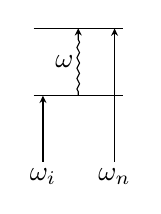
\begin{tikzpicture}[x=0.75pt,y=0.75pt,yscale=-0.5,xscale=0.5]
            %uncomment if require: \path (0,300); %set diagram left start at 0, and has height of 300
            
            %Straight Lines [id:da9549404220987474] 
            \draw    (46,130) -- (131.83,130) ;
            %Straight Lines [id:da7720453820939841] 
            \draw    (46,65) -- (131.83,65) ;
            %Straight Lines [id:da10412337369479152] 
            \draw    (55,133) -- (55,194.28) ;
            \draw [shift={(55,130)}, rotate = 90] [fill={rgb, 255:red, 0; green, 0; blue, 0 }  ][line width=0.08]  [draw opacity=0] (7.14,-3.43) -- (0,0) -- (7.14,3.43) -- (4.74,0) -- cycle    ;
            %Straight Lines [id:da5381448526802415] 
            \draw    (124,68.28) -- (124,194.28) ;
            \draw [shift={(124,65.28)}, rotate = 90] [fill={rgb, 255:red, 0; green, 0; blue, 0 }  ][line width=0.08]  [draw opacity=0] (7.14,-3.43) -- (0,0) -- (7.14,3.43) -- (4.74,0) -- cycle    ;
            %Straight Lines [id:da7027285839417692] 
            \draw    (89,68) -- (89,76) .. controls (90.67,77.67) and (90.67,79.33) .. (89,81) .. controls (87.33,82.67) and (87.33,84.33) .. (89,86) .. controls (90.67,87.67) and (90.67,89.33) .. (89,91) .. controls (87.33,92.67) and (87.33,94.33) .. (89,96) .. controls (90.67,97.67) and (90.67,99.33) .. (89,101) .. controls (87.33,102.67) and (87.33,104.33) .. (89,106) .. controls (90.67,107.67) and (90.67,109.33) .. (89,111) .. controls (87.33,112.67) and (87.33,114.33) .. (89,116) .. controls (90.67,117.67) and (90.67,119.33) .. (89,121) .. controls (87.33,122.67) and (87.33,124.33) .. (89,126) -- (89,129.28) -- (89,129.28) ;
            \draw [shift={(89,65)}, rotate = 90] [fill={rgb, 255:red, 0; green, 0; blue, 0 }  ][line width=0.08]  [draw opacity=0] (7.14,-3.43) -- (0,0) -- (7.14,3.43) -- (4.74,0) -- cycle    ;
            
            % Text Node
            \draw (55,197.28) node [anchor=north] [inner sep=0.75pt]    {$\omega _{i}$};
            % Text Node
            \draw (124,197.28) node [anchor=north] [inner sep=0.75pt]    {$\omega _{n}$};
            % Text Node
            \draw (87,97.14) node [anchor=east] [inner sep=0.75pt]    {$\omega $};
            
            
            \end{tikzpicture}        
    \end{center}
\end{column}

\end{columns}

\vspace{0.5cm}

\begin{columns}

\begin{column}{0.7\textwidth}
    What happens when we consider high order perturbations?
\end{column}

\begin{column}{0.3\textwidth}
\begin{center}
    \vspace{-0.5cm}
    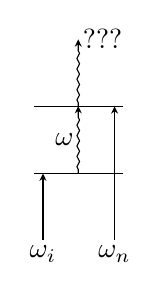
\begin{tikzpicture}[x=0.75pt,y=0.75pt,yscale=-0.5,xscale=0.5]
        %uncomment if require: \path (0,300); %set diagram left start at 0, and has height of 300
        
        %Straight Lines [id:da9549404220987474] 
        \draw    (8,142) -- (93.83,142) ;
        %Straight Lines [id:da7720453820939841] 
        \draw    (8,77) -- (93.83,77) ;
        %Straight Lines [id:da10412337369479152] 
        \draw    (17,145) -- (17,206.28) ;
        \draw [shift={(17,142)}, rotate = 90] [fill={rgb, 255:red, 0; green, 0; blue, 0 }  ][line width=0.08]  [draw opacity=0] (7.14,-3.43) -- (0,0) -- (7.14,3.43) -- (4.74,0) -- cycle    ;
        %Straight Lines [id:da5381448526802415] 
        \draw    (86,80.28) -- (86,206.28) ;
        \draw [shift={(86,77.28)}, rotate = 90] [fill={rgb, 255:red, 0; green, 0; blue, 0 }  ][line width=0.08]  [draw opacity=0] (7.14,-3.43) -- (0,0) -- (7.14,3.43) -- (4.74,0) -- cycle    ;
        %Straight Lines [id:da7027285839417692] 
        \draw    (51,80) -- (51,88) .. controls (52.67,89.67) and (52.67,91.33) .. (51,93) .. controls (49.33,94.67) and (49.33,96.33) .. (51,98) .. controls (52.67,99.67) and (52.67,101.33) .. (51,103) .. controls (49.33,104.67) and (49.33,106.33) .. (51,108) .. controls (52.67,109.67) and (52.67,111.33) .. (51,113) .. controls (49.33,114.67) and (49.33,116.33) .. (51,118) .. controls (52.67,119.67) and (52.67,121.33) .. (51,123) .. controls (49.33,124.67) and (49.33,126.33) .. (51,128) .. controls (52.67,129.67) and (52.67,131.33) .. (51,133) .. controls (49.33,134.67) and (49.33,136.33) .. (51,138) -- (51,141.28) -- (51,141.28) ;
        \draw [shift={(51,77)}, rotate = 90] [fill={rgb, 255:red, 0; green, 0; blue, 0 }  ][line width=0.08]  [draw opacity=0] (7.14,-3.43) -- (0,0) -- (7.14,3.43) -- (4.74,0) -- cycle    ;
        %Straight Lines [id:da6808046989140522] 
        \draw    (51,15.72) -- (51,23.72) .. controls (52.67,25.39) and (52.67,27.05) .. (51,28.72) .. controls (49.33,30.39) and (49.33,32.05) .. (51,33.72) .. controls (52.67,35.39) and (52.67,37.05) .. (51,38.72) .. controls (49.33,40.39) and (49.33,42.05) .. (51,43.72) .. controls (52.67,45.39) and (52.67,47.05) .. (51,48.72) .. controls (49.33,50.39) and (49.33,52.05) .. (51,53.72) .. controls (52.67,55.39) and (52.67,57.05) .. (51,58.72) .. controls (49.33,60.39) and (49.33,62.05) .. (51,63.72) .. controls (52.67,65.39) and (52.67,67.05) .. (51,68.72) .. controls (49.33,70.39) and (49.33,72.05) .. (51,73.72) -- (51,77) -- (51,77) ;
        \draw [shift={(51,12.72)}, rotate = 90] [fill={rgb, 255:red, 0; green, 0; blue, 0 }  ][line width=0.08]  [draw opacity=0] (7.14,-3.43) -- (0,0) -- (7.14,3.43) -- (4.74,0) -- cycle    ;
        
        % Text Node
        \draw (17,209.28) node [anchor=north] [inner sep=0.75pt]    {$\omega _{i}$};
        % Text Node
        \draw (86,209.28) node [anchor=north] [inner sep=0.75pt]    {$\omega _{n}$};
        % Text Node
        \draw (49,109.14) node [anchor=east] [inner sep=0.75pt]    {$\omega $};
        % Text Node
        \draw (53,12.72) node [anchor=west] [inner sep=0.75pt]   [align=left] {???};
        
        
        \end{tikzpicture}        
\end{center} 
\end{column}

\end{columns}

\vspace{0.25cm}

\textbf{Inherently non-equilibrium} The state of photons is a coherent state: $\ket*{\Psi}$ far from any eigenstate!

\end{frame}

\begin{frame}
\frametitle{Overview}

\begin{itemize}
    \item Floquet quasienergies and quasi-stationary states 
    \item Relation with time-dependent perturbation theory and rotating wave approximation (RWA)?
    \item Floquet correction to ARPES 
\end{itemize}

\end{frame}

\begingroup

\title{The Floquet formalism}
\subtitle{Quasi-stationary states and quasienergies}
\author{}
\date{}

\begin{frame}[noframenumbering,plain]
    \titlepage
\end{frame}

\begin{frame}
\frametitle{Periodically driven Hamiltonian: quasi-eigensystem}

\textbf{Floquet theory} $H(t) = H(t + T)$ $\Rightarrow$ 
for every $\ket*{\psi(t)}$, 
\begin{equation*}
    \begin{aligned}
        &\ket*{\psi(t)} = \sum_n c_n \underbrace{\ket*{\psi_n(t)}}_{\text{quasi-stationary basis}} , \quad 
        \ket*{\psi_n(t)} = \ee^{- \ii \varepsilon_n t / \hbar} \underbrace{
            \ket*{\Phi_n(t)}
        }_\text{period is $T$} ,
    \end{aligned}
\end{equation*}

\begin{itemize}
    \item Time evolution of arbitrary states $\Leftrightarrow$ $\{\ket*{\psi_n(t)}\}$
    %\item $\mathcal{H} \otimes \{m= \ldots, -1, 0, 1, \ldots \}$: \concept{extended Hilbert space}
    \item $\{\psi_n(t)\}$: \concept{quasi-stationary states}
    \item $\{\varepsilon_n\}$: \concept{quasienergies} (c.f. crystal momentum)
\end{itemize}

\vspace{0.5cm}

\textbf{Our task} How to find $\{ \psi_n(t) \}$ and $\{ \varepsilon_n \}$?

\begin{equation*}
    \ket*{\Phi_n(t)} = \underbrace{\sum_m \ee^{- \ii m \omega t} \ket*{\phi_n^{(m)}}}_{\text{discrete Fourier series}} , \quad 
    \omega = 2\pi / T. 
\end{equation*}


\end{frame}

\begin{frame}
\frametitle{Floquet effective Hamiltonian}

\textbf{Our task} A Hamiltonian for $\{ \phi_n^{(m)} \}$ and $\{ \varepsilon_n \}$? 

\[
    \begin{aligned}
        &\quad 
        \ii \hbar \partial_t \underbrace{\sum_{m} \ee^{-\ii (\varepsilon_n + m \hbar \omega) t / \hbar} \ket*{\phi_n^{(m)}}}_{\ket*{\psi_n(t)}}  = \underbrace{H(t)}_{\eqqcolon \sum_m \ee^{- \ii m \omega t} H^{(m)}} \ket*{\psi_n(t)} \\
        &\Rightarrow (\varepsilon_n + m \hbar \omega) \ket*{\phi_n^{(m)}} = \sum_{m'} H^{(m - m')} \ket*{\phi^{(m')}_n} \\
        &\uncover<2>{
            \Rightarrow \boxed{\varepsilon_n \ket*{\phi_n^{(m)}}
            = \sum_{m'} (H^{(m-m')} - m \hbar \omega \delta_{mm'})  \ket*{\phi_n^{(m')}}.}
        }
    \end{aligned}
\]
\uncover<2->{
    \textbf{Floquet effective Hamiltonian} Indeed we have a Hamiltonian!!
}


\end{frame}

\begin{frame}
\frametitle{Floquet effective Hamiltonian}

$\varepsilon_n$, $(\cdots , \ket*{\phi_n^{(-1)}} , \ket*{\phi_n^{(0)}} , \ket*{\phi_n^{(1)}} , \cdots)$ are obtained by diagonalizing
\[
    \begin{pNiceMatrix}[first-row,first-col]
        &        & m'=-2 & m'=-1 & m'=0 & m'=1 \\
        &        &     & \vdots & \vdots & \\
   m=-2 &        & H^{(0)} + 2 \hbar \omega   & H^{(-1)}   & H^{(-2)}   & H^{(-3)} &  \\
   m=-1 & \hdots & H^{(1)}   & H^{(0)} + \hbar \omega  & H^{(-1)}   & H^{(-2)} & \hdots \\
   m=0  & \hdots & H^{(2)}   & H^{(1)}   & H^{(0)}   & H^{(-1)} & \hdots  \\
   m=1  &        & H^{(3)}   & H^{(2)}   & H^{(1)}   & H^{(0)} - \hbar \omega &  \\
       &        &     & \vdots & \vdots & \\
   \end{pNiceMatrix}
\]

\begin{itemize}
    \item Each ``element'' is a matrix on $\mathcal{H}$
    \item $H^{(0)}$: $H$ without driving; 
    $H^{(m)}$: driving with frequency $m \omega$
    \item $H^{\text{Floquet}}$ is on the extended Hilbert space $\mathcal{H} \otimes \{m= \ldots, -1, 0, 1, \ldots \}$
\end{itemize}

\end{frame}

\begin{frame}
\frametitle{Floquet Brillouin zone}

\vspace{0.3cm}

\begin{columns}

\begin{column}{0.6\textwidth}
    \begin{minipage}{\columnwidth}
        \textbf{Redundancy in $H^{\text{Floquet}}$} The number of independent quasienergies is not really multiplied by Floquet subspaces.
        \[
            \underbrace{
                \ee^{- \ii (\varepsilon_n / \hbar + m \omega) t} \underbrace{\ee^{\ii m \omega t} \ket*{\Phi_n(t)}}_{\text{still periodic!}}
            }_\text{both $\varepsilon_n$ and $\varepsilon_n + m \hbar \omega$ are its quasienergies}
        \]
    \end{minipage}
\end{column}

\begin{column}{0.39\textwidth}
    \begin{minipage}{\columnwidth}
        \centering
        \only<1>{
            
\begin{tikzpicture}[x=0.75pt,y=0.75pt,yscale=-0.6,xscale=0.6]
                %uncomment if require: \path (0,300); %set diagram left start at 0, and has height of 300
                
                %Straight Lines [id:da8729664532403207] 
                \draw [color={rgb, 255:red, 189; green, 16; blue, 224 }  ,draw opacity=1 ][fill={rgb, 255:red, 189; green, 16; blue, 224 }  ,fill opacity=1 ][line width=2.25]    (43,232) -- (155.83,232) ;
                %Straight Lines [id:da26798948442984627] 
                \draw [color={rgb, 255:red, 80; green, 227; blue, 194 }  ,draw opacity=1 ][fill={rgb, 255:red, 74; green, 144; blue, 226 }  ,fill opacity=1 ][line width=2.25]    (43,122) -- (156.25,122) ;
                %Straight Lines [id:da3856603960762994] 
                \draw [color={rgb, 255:red, 184; green, 233; blue, 134 }  ,draw opacity=1 ][line width=2.25]    (43.42,37.73) -- (156.25,37.73) ;
                
                
                
                
                \end{tikzpicture}
        }
        \only<2>{
            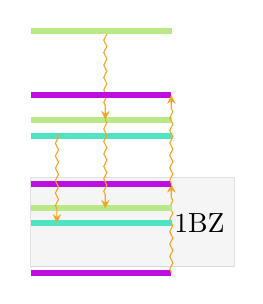
\begin{tikzpicture}[x=0.75pt,y=0.75pt,yscale=-0.6,xscale=0.6]
                %uncomment if require: \path (0,300); %set diagram left start at 0, and has height of 300
                
                %Shape: Rectangle [id:dp7298301359950772] 
                \draw  [color={rgb, 255:red, 155; green, 155; blue, 155 }  ,draw opacity=0.3 ][fill={rgb, 255:red, 155; green, 155; blue, 155 }  ,fill opacity=0.1 ] (42.92,155.73) -- (206.25,155.73) -- (206.25,227.11) -- (42.92,227.11) -- cycle ;
                %Straight Lines [id:da9181682037828782] 
                \draw [color={rgb, 255:red, 189; green, 16; blue, 224 }  ,draw opacity=1 ][fill={rgb, 255:red, 189; green, 16; blue, 224 }  ,fill opacity=1 ][line width=2.25]    (43,232) -- (155.83,232) ;
                %Straight Lines [id:da7127792152745307] 
                \draw [color={rgb, 255:red, 245; green, 166; blue, 35 }  ,draw opacity=1 ]   (155.83,163.61) -- (155.83,171.61) .. controls (157.5,173.28) and (157.5,174.94) .. (155.83,176.61) .. controls (154.16,178.28) and (154.16,179.94) .. (155.83,181.61) .. controls (157.5,183.28) and (157.5,184.94) .. (155.83,186.61) .. controls (154.16,188.28) and (154.16,189.94) .. (155.83,191.61) .. controls (157.5,193.28) and (157.5,194.94) .. (155.83,196.61) .. controls (154.16,198.28) and (154.16,199.94) .. (155.83,201.61) .. controls (157.5,203.28) and (157.5,204.94) .. (155.83,206.61) .. controls (154.16,208.28) and (154.16,209.94) .. (155.83,211.61) .. controls (157.5,213.28) and (157.5,214.94) .. (155.83,216.61) .. controls (154.16,218.28) and (154.16,219.94) .. (155.83,221.61) .. controls (157.5,223.28) and (157.5,224.94) .. (155.83,226.61) .. controls (154.16,228.28) and (154.16,229.94) .. (155.83,231.61) -- (155.83,232) -- (155.83,232) ;
                \draw [shift={(155.83,160.61)}, rotate = 90] [fill={rgb, 255:red, 245; green, 166; blue, 35 }  ,fill opacity=1 ][line width=0.08]  [draw opacity=0] (7.14,-3.43) -- (0,0) -- (7.14,3.43) -- (4.74,0) -- cycle    ;
                %Straight Lines [id:da6882390234213356] 
                \draw [color={rgb, 255:red, 80; green, 227; blue, 194 }  ,draw opacity=1 ][fill={rgb, 255:red, 74; green, 144; blue, 226 }  ,fill opacity=1 ][line width=2.25]    (43.5,192) -- (156.33,192) ;
                %Straight Lines [id:da0739201384454593] 
                \draw [color={rgb, 255:red, 184; green, 233; blue, 134 }  ,draw opacity=1 ][line width=2.25]    (43.5,180) -- (156.33,180) ;
                %Straight Lines [id:da9326208918546175] 
                \draw [color={rgb, 255:red, 189; green, 16; blue, 224 }  ,draw opacity=1 ][fill={rgb, 255:red, 189; green, 16; blue, 224 }  ,fill opacity=1 ][line width=2.25]    (43,160.61) -- (155.83,160.61) ;
                %Straight Lines [id:da41986982307748066] 
                \draw [color={rgb, 255:red, 80; green, 227; blue, 194 }  ,draw opacity=1 ][fill={rgb, 255:red, 74; green, 144; blue, 226 }  ,fill opacity=1 ][line width=2.25]    (43,122) -- (156.25,122) ;
                %Straight Lines [id:da8598211610411646] 
                \draw [color={rgb, 255:red, 245; green, 166; blue, 35 }  ,draw opacity=1 ]   (64,120.61) .. controls (65.67,122.28) and (65.67,123.94) .. (64,125.61) .. controls (62.33,127.28) and (62.33,128.94) .. (64,130.61) .. controls (65.67,132.28) and (65.67,133.94) .. (64,135.61) .. controls (62.33,137.28) and (62.33,138.94) .. (64,140.61) .. controls (65.67,142.28) and (65.67,143.94) .. (64,145.61) .. controls (62.33,147.28) and (62.33,148.94) .. (64,150.61) .. controls (65.67,152.28) and (65.67,153.94) .. (64,155.61) .. controls (62.33,157.28) and (62.33,158.94) .. (64,160.61) .. controls (65.67,162.28) and (65.67,163.94) .. (64,165.61) .. controls (62.33,167.28) and (62.33,168.94) .. (64,170.61) .. controls (65.67,172.28) and (65.67,173.94) .. (64,175.61) .. controls (62.33,177.28) and (62.33,178.94) .. (64,180.61) -- (64,181) -- (64,189) ;
                \draw [shift={(64,192)}, rotate = 270] [fill={rgb, 255:red, 245; green, 166; blue, 35 }  ,fill opacity=1 ][line width=0.08]  [draw opacity=0] (7.14,-3.43) -- (0,0) -- (7.14,3.43) -- (4.74,0) -- cycle    ;
                %Straight Lines [id:da011513546790421492] 
                \draw [color={rgb, 255:red, 184; green, 233; blue, 134 }  ,draw opacity=1 ][line width=2.25]    (43.42,109.11) -- (156.25,109.11) ;
                %Straight Lines [id:da8767692107987499] 
                \draw [color={rgb, 255:red, 245; green, 166; blue, 35 }  ,draw opacity=1 ]   (102.83,109.11) .. controls (104.5,110.78) and (104.5,112.44) .. (102.83,114.11) .. controls (101.16,115.78) and (101.16,117.44) .. (102.83,119.11) .. controls (104.5,120.78) and (104.5,122.44) .. (102.83,124.11) .. controls (101.16,125.78) and (101.16,127.44) .. (102.83,129.11) .. controls (104.5,130.78) and (104.5,132.44) .. (102.83,134.11) .. controls (101.16,135.78) and (101.16,137.44) .. (102.83,139.11) .. controls (104.5,140.78) and (104.5,142.44) .. (102.83,144.11) .. controls (101.16,145.78) and (101.16,147.44) .. (102.83,149.11) .. controls (104.5,150.78) and (104.5,152.44) .. (102.83,154.11) .. controls (101.16,155.78) and (101.16,157.44) .. (102.83,159.11) .. controls (104.5,160.78) and (104.5,162.44) .. (102.83,164.11) .. controls (101.16,165.78) and (101.16,167.44) .. (102.83,169.11) -- (102.83,169.5) -- (102.83,177.5) ;
                \draw [shift={(102.83,180.5)}, rotate = 270] [fill={rgb, 255:red, 245; green, 166; blue, 35 }  ,fill opacity=1 ][line width=0.08]  [draw opacity=0] (7.14,-3.43) -- (0,0) -- (7.14,3.43) -- (4.74,0) -- cycle    ;
                %Straight Lines [id:da4354918972699331] 
                \draw [color={rgb, 255:red, 245; green, 166; blue, 35 }  ,draw opacity=1 ]   (102.83,37.73) .. controls (104.5,39.4) and (104.5,41.06) .. (102.83,42.73) .. controls (101.16,44.4) and (101.16,46.06) .. (102.83,47.73) .. controls (104.5,49.4) and (104.5,51.06) .. (102.83,52.73) .. controls (101.16,54.4) and (101.16,56.06) .. (102.83,57.73) .. controls (104.5,59.4) and (104.5,61.06) .. (102.83,62.73) .. controls (101.16,64.4) and (101.16,66.06) .. (102.83,67.73) .. controls (104.5,69.4) and (104.5,71.06) .. (102.83,72.73) .. controls (101.16,74.4) and (101.16,76.06) .. (102.83,77.73) .. controls (104.5,79.4) and (104.5,81.06) .. (102.83,82.73) .. controls (101.16,84.4) and (101.16,86.06) .. (102.83,87.73) .. controls (104.5,89.4) and (104.5,91.06) .. (102.83,92.73) .. controls (101.16,94.4) and (101.16,96.06) .. (102.83,97.73) -- (102.83,98.11) -- (102.83,106.11) ;
                \draw [shift={(102.83,109.11)}, rotate = 270] [fill={rgb, 255:red, 245; green, 166; blue, 35 }  ,fill opacity=1 ][line width=0.08]  [draw opacity=0] (7.14,-3.43) -- (0,0) -- (7.14,3.43) -- (4.74,0) -- cycle    ;
                %Straight Lines [id:da5649695485657895] 
                \draw [color={rgb, 255:red, 184; green, 233; blue, 134 }  ,draw opacity=1 ][line width=2.25]    (43.42,37.73) -- (156.25,37.73) ;
                %Straight Lines [id:da7954828909315641] 
                \draw [color={rgb, 255:red, 189; green, 16; blue, 224 }  ,draw opacity=1 ][fill={rgb, 255:red, 189; green, 16; blue, 224 }  ,fill opacity=1 ][line width=2.25]    (43,89.23) -- (155.83,89.23) ;
                %Straight Lines [id:da6145585950854873] 
                \draw [color={rgb, 255:red, 245; green, 166; blue, 35 }  ,draw opacity=1 ]   (155.83,92.23) -- (155.83,100.23) .. controls (157.5,101.9) and (157.5,103.56) .. (155.83,105.23) .. controls (154.16,106.9) and (154.16,108.56) .. (155.83,110.23) .. controls (157.5,111.9) and (157.5,113.56) .. (155.83,115.23) .. controls (154.16,116.9) and (154.16,118.56) .. (155.83,120.23) .. controls (157.5,121.9) and (157.5,123.56) .. (155.83,125.23) .. controls (154.16,126.9) and (154.16,128.56) .. (155.83,130.23) .. controls (157.5,131.9) and (157.5,133.56) .. (155.83,135.23) .. controls (154.16,136.9) and (154.16,138.56) .. (155.83,140.23) .. controls (157.5,141.9) and (157.5,143.56) .. (155.83,145.23) .. controls (154.16,146.9) and (154.16,148.56) .. (155.83,150.23) .. controls (157.5,151.9) and (157.5,153.56) .. (155.83,155.23) .. controls (154.16,156.9) and (154.16,158.56) .. (155.83,160.23) -- (155.83,160.61) -- (155.83,160.61) ;
                \draw [shift={(155.83,89.23)}, rotate = 90] [fill={rgb, 255:red, 245; green, 166; blue, 35 }  ,fill opacity=1 ][line width=0.08]  [draw opacity=0] (7.14,-3.43) -- (0,0) -- (7.14,3.43) -- (4.74,0) -- cycle    ;
                
                % Text Node
                \draw (200.75,191.8) node [anchor=east] [inner sep=0.75pt]   [align=left] {1BZ};
                
                
                \end{tikzpicture}               
        }
    \end{minipage}
\end{column}

\end{columns}

\only<2>{
    \vspace{0.5cm}

    So only \emph{one} energy Brillouin zone is needed.
    
    \textbf{The number of independent quasi-stationary states $= \dim \mathcal{H}$}
    
    \vspace{0.5cm}
    
    But all $\phi_n^{(m)}$ are all needed to decide $\ket*{\psi_n(t)}$.
}

\end{frame}

\endgroup

\begingroup

\title{Floquet formalism in eyes of other formalisms}
\subtitle{``full'' Floquet theory, perturbation theory, and RWA}
\author{}
\date{}

\begin{frame}[noframenumbering,plain]
    \titlepage
\end{frame}

\begin{frame}
    \frametitle{Floquet formalism in hierarchy of approximations}
    
    \textbf{Other ways to describe periodic driving}
    
    \begin{itemize}
        \item Time-dependent perturbation theory (TD-PT)
        \item Rotating wave approximation (RWA)
    \end{itemize}
    
    
    \begin{center}
        \small
        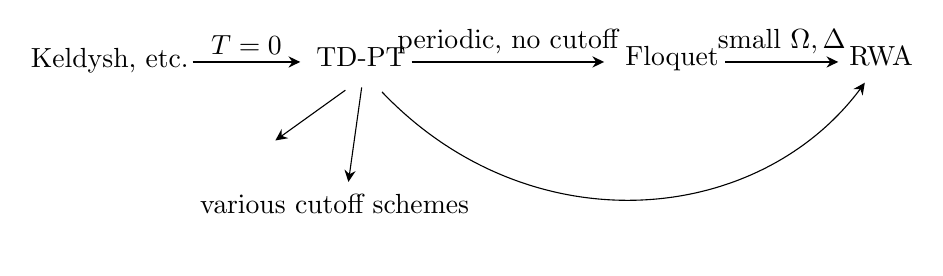
\begin{tikzpicture}[x=0.75pt,y=0.75pt,yscale=-0.8,xscale=0.8]
            %uncomment if require: \path (0,300); %set diagram left start at 0, and has height of 300
            
            %Straight Lines [id:da3808102939067066] 
            \draw    (118,88) -- (179.83,88) ;
            \draw [shift={(182.83,88)}, rotate = 180] [fill={rgb, 255:red, 0; green, 0; blue, 0 }  ][line width=0.08]  [draw opacity=0] (7.14,-3.43) -- (0,0) -- (7.14,3.43) -- (4.74,0) -- cycle    ;
            %Straight Lines [id:da17889125564532904] 
            \draw    (210,105) -- (170.27,133.53) ;
            \draw [shift={(167.83,135.28)}, rotate = 324.32] [fill={rgb, 255:red, 0; green, 0; blue, 0 }  ][line width=0.08]  [draw opacity=0] (7.14,-3.43) -- (0,0) -- (7.14,3.43) -- (4.74,0) -- cycle    ;
            %Straight Lines [id:da8600528475726741] 
            \draw    (219.83,103.28) -- (212.25,157.31) ;
            \draw [shift={(211.83,160.28)}, rotate = 277.99] [fill={rgb, 255:red, 0; green, 0; blue, 0 }  ][line width=0.08]  [draw opacity=0] (7.14,-3.43) -- (0,0) -- (7.14,3.43) -- (4.74,0) -- cycle    ;
            %Straight Lines [id:da9418458232454647] 
            \draw    (249.83,88) -- (362.83,88) ;
            \draw [shift={(365.83,88)}, rotate = 180] [fill={rgb, 255:red, 0; green, 0; blue, 0 }  ][line width=0.08]  [draw opacity=0] (7.14,-3.43) -- (0,0) -- (7.14,3.43) -- (4.74,0) -- cycle    ;
            %Straight Lines [id:da024612001433695463] 
            \draw    (438.83,88) -- (503.83,88) ;
            \draw [shift={(506.83,88)}, rotate = 180] [fill={rgb, 255:red, 0; green, 0; blue, 0 }  ][line width=0.08]  [draw opacity=0] (7.14,-3.43) -- (0,0) -- (7.14,3.43) -- (4.74,0) -- cycle    ;
            %Curve Lines [id:da020758323785619925] 
            \draw    (232,106) .. controls (321.38,199.81) and (460.43,187.41) .. (521.91,101.78) ;
            \draw [shift={(522.83,100.48)}, rotate = 125.1] [fill={rgb, 255:red, 0; green, 0; blue, 0 }  ][line width=0.08]  [draw opacity=0] (7.14,-3.43) -- (0,0) -- (7.14,3.43) -- (4.74,0) -- cycle    ;
            
            % Text Node
            \draw (19,78) node [anchor=north west][inner sep=0.75pt]   [align=left] {Keldysh, etc.};
            % Text Node
            \draw (191,78) node [anchor=north west][inner sep=0.75pt]   [align=left] {TD-PT};
            % Text Node
            \draw (150.42,85) node [anchor=south] [inner sep=0.75pt]    {$T=0$};
            % Text Node
            \draw (121,166) node [anchor=north west][inner sep=0.75pt]   [align=left] {various cutoff schemes};
            % Text Node
            \draw (307.83,85) node [anchor=south] [inner sep=0.75pt]   [align=left] {periodic, no cutoff};
            % Text Node
            \draw (377,77) node [anchor=north west][inner sep=0.75pt]   [align=left] {Floquet};
            % Text Node
            \draw (512,77) node [anchor=north west][inner sep=0.75pt]   [align=left] {RWA};
            % Text Node
            \draw (472.83,85) node [anchor=south] [inner sep=0.75pt]   [align=left] {small $\displaystyle \Omega ,\Delta $};
            
            
            \end{tikzpicture}        
    \end{center}    
    
    
\end{frame}

\begin{frame}
\frametitle{Floquet formalism v.s. TD-PT}

Response from time-dependent perturbation theory
$=$ response from $T=0$ Feynman diagrams. 

\textbf{Example: first-order PT = Lindhard response function}
\vspace{-0.4cm}
\[
    \small
    \expval*{\mu^{(1)}} = \mueg\underbrace{ \Omega}_{\text{Rabi freq.}} \left(
        \frac{\Omega}{\omegaeg - \omega} \ee^{- \ii \omega t}
        + \frac{\Omega}{\omegaeg + \omega} \ee^{\ii \omega t} + \text{h.c.}
    \right) = \begin{gathered}
        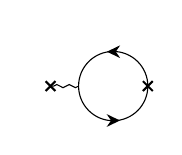
\begin{tikzpicture}[x=0.75pt,y=0.75pt,yscale=-0.6,xscale=0.6, baseline=(XXXX.south) ]
            \draw    ($(current bounding box.center)+(0,0.3em)$) node [anchor=south] (XXXX) {};
            %Shape: Circle [id:dp9093318337648062] 
            \draw   (33.47,35.64) .. controls (33.47,20.28) and (45.92,7.83) .. (61.28,7.83) .. controls (76.63,7.83) and (89.08,20.28) .. (89.08,35.64) .. controls (89.08,51) and (76.63,63.45) .. (61.28,63.45) .. controls (45.92,63.45) and (33.47,51) .. (33.47,35.64) -- cycle ;
            %Straight Lines [id:da7974609162256947] 
            \draw    (58.96,8.03) ;
            \draw [shift={(56.21,8.03)}, rotate = 360] [fill={rgb, 255:red, 0; green, 0; blue, 0 }  ][line width=0.08]  [draw opacity=0] (10.72,-5.15) -- (0,0) -- (10.72,5.15) -- (7.12,0) -- cycle    ;
            %Straight Lines [id:da9935047452925077] 
            \draw    (64.21,63.28) ;
            \draw [shift={(66.71,63.28)}, rotate = 180] [fill={rgb, 255:red, 0; green, 0; blue, 0 }  ][line width=0.08]  [draw opacity=0] (10.72,-5.15) -- (0,0) -- (10.72,5.15) -- (7.12,0) -- cycle    ;
            %Straight Lines [id:da661786151633333] 
            \draw    (33.47,35.64) .. controls (31.8,37.31) and (30.14,37.31) .. (28.47,35.64) .. controls (26.8,33.97) and (25.14,33.97) .. (23.47,35.64) .. controls (21.8,37.31) and (20.14,37.31) .. (18.47,35.64) .. controls (16.8,33.97) and (15.14,33.97) .. (13.47,35.64) -- (10.96,35.64) -- (10.96,35.64) ;
            \draw [shift={(10.96,35.64)}, rotate = 225] [color={rgb, 255:red, 0; green, 0; blue, 0 }  ][line width=0.75]    (-5.59,0) -- (5.59,0)(0,5.59) -- (0,-5.59)   ;
            %Straight Lines [id:da28063751054916297] 
            \draw    (89.08,35.64) ;
            \draw [shift={(89.08,35.64)}, rotate = 45] [color={rgb, 255:red, 0; green, 0; blue, 0 }  ][line width=0.75]    (-5.59,0) -- (5.59,0)(0,5.59) -- (0,-5.59)   ;
            \end{tikzpicture}
    \end{gathered}
\]

\only<2>{
    And when we sum over all of them\dots
    \[
        
\begin{tikzpicture}[x=0.75pt,y=0.75pt,yscale=-1,xscale=1, baseline=(XXXX.south) ]
            \path (0,64);\path (16.666667938232422,0);\draw    ($(current bounding box.center)+(0,0.3em)$) node [anchor=south] (XXXX) {};
            %Straight Lines [id:da8412536094935157] 
            \draw [color={rgb, 255:red, 74; green, 144; blue, 226 }  ,draw opacity=1 ][line width=2.25]    (7.83,7.11) -- (7.83,56.11) ;
            \draw [shift={(7.83,23.91)}, rotate = 90] [fill={rgb, 255:red, 74; green, 144; blue, 226 }  ,fill opacity=1 ][line width=0.08]  [draw opacity=0] (10.36,-4.98) -- (0,0) -- (10.36,4.98) -- (6.88,0) -- cycle    ;
            \end{tikzpicture}
            =\tikzset{every picture/.style={line width=0.75pt}} %set default line width to 0.75pt        
            \begin{tikzpicture}[x=0.75pt,y=0.75pt,yscale=-1,xscale=1, baseline=(XXXX.south) ]
            \path (0,64);\path (16.666667938232422,0);\draw    ($(current bounding box.center)+(0,0.3em)$) node [anchor=south] (XXXX) {};
            %Straight Lines [id:da2662290946504795] 
            \draw [color={rgb, 255:red, 74; green, 144; blue, 226 }  ,draw opacity=1 ][line width=0.75]    (7.83,7.11) -- (7.83,56.11) ;
            \draw [shift={(7.83,27.51)}, rotate = 90] [fill={rgb, 255:red, 74; green, 144; blue, 226 }  ,fill opacity=1 ][line width=0.08]  [draw opacity=0] (7.14,-3.43) -- (0,0) -- (7.14,3.43) -- (4.74,0) -- cycle    ;
            \end{tikzpicture}
            +\tikzset{every picture/.style={line width=0.75pt}} %set default line width to 0.75pt        
            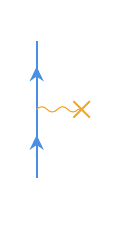
\begin{tikzpicture}[x=0.75pt,y=0.75pt,yscale=-1,xscale=1, baseline=(XXXX.south) ]
            \path (0,82);\path (34.25,0);\draw    ($(current bounding box.center)+(0,0.3em)$) node [anchor=south] (XXXX) {};
            %Straight Lines [id:da22106981645682056] 
            \draw [color={rgb, 255:red, 74; green, 144; blue, 226 }  ,draw opacity=1 ][line width=0.75]    (4.33,39.36) -- (4.33,72.36) ;
            \draw [shift={(4.33,51.76)}, rotate = 90] [fill={rgb, 255:red, 74; green, 144; blue, 226 }  ,fill opacity=1 ][line width=0.08]  [draw opacity=0] (7.14,-3.43) -- (0,0) -- (7.14,3.43) -- (4.74,0) -- cycle    ;
            %Straight Lines [id:da5240738024395817] 
            \draw [color={rgb, 255:red, 74; green, 144; blue, 226 }  ,draw opacity=1 ][line width=0.75]    (4.33,6.36) -- (4.33,39.36) ;
            \draw [shift={(4.33,18.76)}, rotate = 90] [fill={rgb, 255:red, 74; green, 144; blue, 226 }  ,fill opacity=1 ][line width=0.08]  [draw opacity=0] (7.14,-3.43) -- (0,0) -- (7.14,3.43) -- (4.74,0) -- cycle    ;
            %Straight Lines [id:da7341318154975915] 
            \draw [color={rgb, 255:red, 245; green, 166; blue, 35 }  ,draw opacity=1 ]   (4.33,39.36) .. controls (6,37.69) and (7.66,37.69) .. (9.33,39.36) .. controls (11,41.03) and (12.66,41.03) .. (14.33,39.36) .. controls (16,37.69) and (17.66,37.69) .. (19.33,39.36) .. controls (21,41.03) and (22.66,41.03) .. (24.33,39.36) -- (25.98,39.36) -- (25.98,39.36) ;
            \draw [shift={(25.98,39.36)}, rotate = 45] [color={rgb, 255:red, 245; green, 166; blue, 35 }  ,draw opacity=1 ][line width=0.75]    (-5.59,0) -- (5.59,0)(0,5.59) -- (0,-5.59)   ;
            \end{tikzpicture}
            +\tikzset{every picture/.style={line width=0.75pt}} %set default line width to 0.75pt        
            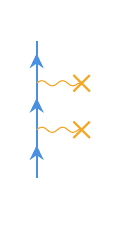
\begin{tikzpicture}[x=0.75pt,y=0.75pt,yscale=-1,xscale=1, baseline=(XXXX.south) ]
            \path (0,82);\path (34.25,0);\draw    ($(current bounding box.center)+(0,0.3em)$) node [anchor=south] (XXXX) {};
            %Straight Lines [id:da8161777701105761] 
            \draw [color={rgb, 255:red, 74; green, 144; blue, 226 }  ,draw opacity=1 ][line width=0.75]    (4.33,49.2) -- (4.33,72.36) ;
            \draw [shift={(4.33,56.68)}, rotate = 90] [fill={rgb, 255:red, 74; green, 144; blue, 226 }  ,fill opacity=1 ][line width=0.08]  [draw opacity=0] (7.14,-3.43) -- (0,0) -- (7.14,3.43) -- (4.74,0) -- cycle    ;
            %Straight Lines [id:da2788545187674776] 
            \draw [color={rgb, 255:red, 74; green, 144; blue, 226 }  ,draw opacity=1 ][line width=0.75]    (4.33,6.36) -- (4.33,26.78) ;
            \draw [shift={(4.33,12.47)}, rotate = 90] [fill={rgb, 255:red, 74; green, 144; blue, 226 }  ,fill opacity=1 ][line width=0.08]  [draw opacity=0] (7.14,-3.43) -- (0,0) -- (7.14,3.43) -- (4.74,0) -- cycle    ;
            %Straight Lines [id:da49547361269120516] 
            \draw [color={rgb, 255:red, 245; green, 166; blue, 35 }  ,draw opacity=1 ]   (4.33,26.78) .. controls (6,25.11) and (7.66,25.11) .. (9.33,26.78) .. controls (11,28.45) and (12.66,28.45) .. (14.33,26.78) .. controls (16,25.11) and (17.66,25.11) .. (19.33,26.78) .. controls (21,28.45) and (22.66,28.45) .. (24.33,26.78) -- (25.98,26.78) -- (25.98,26.78) ;
            \draw [shift={(25.98,26.78)}, rotate = 45] [color={rgb, 255:red, 245; green, 166; blue, 35 }  ,draw opacity=1 ][line width=0.75]    (-5.59,0) -- (5.59,0)(0,5.59) -- (0,-5.59)   ;
            %Straight Lines [id:da12325027121000054] 
            \draw [color={rgb, 255:red, 74; green, 144; blue, 226 }  ,draw opacity=1 ][line width=0.75]    (4.33,26.78) -- (4.33,49.2) ;
            \draw [shift={(4.33,33.89)}, rotate = 90] [fill={rgb, 255:red, 74; green, 144; blue, 226 }  ,fill opacity=1 ][line width=0.08]  [draw opacity=0] (7.14,-3.43) -- (0,0) -- (7.14,3.43) -- (4.74,0) -- cycle    ;
            %Straight Lines [id:da6221500517164411] 
            \draw [color={rgb, 255:red, 245; green, 166; blue, 35 }  ,draw opacity=1 ]   (4.33,49.2) .. controls (6,47.53) and (7.66,47.53) .. (9.33,49.2) .. controls (11,50.87) and (12.66,50.87) .. (14.33,49.2) .. controls (16,47.53) and (17.66,47.53) .. (19.33,49.2) .. controls (21,50.87) and (22.66,50.87) .. (24.33,49.2) -- (25.98,49.2) -- (25.98,49.2) ;
            \draw [shift={(25.98,49.2)}, rotate = 45] [color={rgb, 255:red, 245; green, 166; blue, 35 }  ,draw opacity=1 ][line width=0.75]    (-5.59,0) -- (5.59,0)(0,5.59) -- (0,-5.59)   ;
            \end{tikzpicture}
            +\cdots
    \]
}

\uncover<3->{
    \textbf{$H^{\text{Floquet}}$ is the non-equilibrium self-energy}

    \[
        
\begin{tikzpicture}[x=0.75pt,y=0.75pt,yscale=-1,xscale=1, baseline=(XXXX.south) ]
            \path (0,64);\path (16.666667938232422,0);\draw    ($(current bounding box.center)+(0,0.3em)$) node [anchor=south] (XXXX) {};
            %Straight Lines [id:da9841518915215031] 
            \draw [color={rgb, 255:red, 74; green, 144; blue, 226 }  ,draw opacity=1 ][line width=2.25]    (7.83,7.11) -- (7.83,56.11) ;
            \draw [shift={(7.83,23.91)}, rotate = 90] [fill={rgb, 255:red, 74; green, 144; blue, 226 }  ,fill opacity=1 ][line width=0.08]  [draw opacity=0] (10.36,-4.98) -- (0,0) -- (10.36,4.98) -- (6.88,0) -- cycle    ;
            \end{tikzpicture}
            =\tikzset{every picture/.style={line width=0.75pt}} %set default line width to 0.75pt        
            \begin{tikzpicture}[x=0.75pt,y=0.75pt,yscale=-1,xscale=1, baseline=(XXXX.south) ]
            \path (0,64);\path (16.666667938232422,0);\draw    ($(current bounding box.center)+(0,0.3em)$) node [anchor=south] (XXXX) {};
            %Straight Lines [id:da14865900251827657] 
            \draw [color={rgb, 255:red, 74; green, 144; blue, 226 }  ,draw opacity=1 ][line width=0.75]    (7.83,7.11) -- (7.83,56.11) ;
            \draw [shift={(7.83,27.51)}, rotate = 90] [fill={rgb, 255:red, 74; green, 144; blue, 226 }  ,fill opacity=1 ][line width=0.08]  [draw opacity=0] (7.14,-3.43) -- (0,0) -- (7.14,3.43) -- (4.74,0) -- cycle    ;
            \end{tikzpicture}
            +\tikzset{every picture/.style={line width=0.75pt}} %set default line width to 0.75pt        
            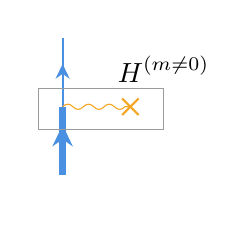
\begin{tikzpicture}[x=0.75pt,y=0.75pt,yscale=-1,xscale=1, baseline=(XXXX.south) ]
            \path (0,82);\path (94.33333587646484,0);\draw    ($(current bounding box.center)+(0,0.3em)$) node [anchor=south] (XXXX) {};
            %Straight Lines [id:da0005960179652220177] 
            \draw [color={rgb, 255:red, 74; green, 144; blue, 226 }  ,draw opacity=1 ][line width=2.25]    (16.83,38.11) -- (16.83,71.11) ;
            \draw [shift={(16.83,46.91)}, rotate = 90] [fill={rgb, 255:red, 74; green, 144; blue, 226 }  ,fill opacity=1 ][line width=0.08]  [draw opacity=0] (10.36,-4.98) -- (0,0) -- (10.36,4.98) -- (6.88,0) -- cycle    ;
            %Straight Lines [id:da537794110388885] 
            \draw [color={rgb, 255:red, 74; green, 144; blue, 226 }  ,draw opacity=1 ][line width=0.75]    (16.83,5.11) -- (16.83,38.11) ;
            \draw [shift={(16.83,17.51)}, rotate = 90] [fill={rgb, 255:red, 74; green, 144; blue, 226 }  ,fill opacity=1 ][line width=0.08]  [draw opacity=0] (7.14,-3.43) -- (0,0) -- (7.14,3.43) -- (4.74,0) -- cycle    ;
            %Straight Lines [id:da5838170117024906] 
            \draw [color={rgb, 255:red, 245; green, 166; blue, 35 }  ,draw opacity=1 ]   (16.83,38.11) .. controls (18.5,36.44) and (20.16,36.44) .. (21.83,38.11) .. controls (23.5,39.78) and (25.16,39.78) .. (26.83,38.11) .. controls (28.5,36.44) and (30.16,36.44) .. (31.83,38.11) .. controls (33.5,39.78) and (35.16,39.78) .. (36.83,38.11) .. controls (38.5,36.44) and (40.16,36.44) .. (41.83,38.11) .. controls (43.5,39.78) and (45.16,39.78) .. (46.83,38.11) -- (49.48,38.11) -- (49.48,38.11) ;
            \draw [shift={(49.48,38.11)}, rotate = 45] [color={rgb, 255:red, 245; green, 166; blue, 35 }  ,draw opacity=1 ][line width=0.75]    (-5.59,0) -- (5.59,0)(0,5.59) -- (0,-5.59)   ;
            %Shape: Rectangle [id:dp4375384855512545] 
            \draw  [color={rgb, 255:red, 155; green, 155; blue, 155 }  ,draw opacity=1 ] (5.33,29.11) -- (65.48,29.11) -- (65.48,49.11) -- (5.33,49.11) -- cycle ;
            % Text Node
            \draw (65.48,27.61) node [anchor=south] [inner sep=0.75pt]   [align=left] {$\displaystyle H^{( m\neq 0)}$};
            \end{tikzpicture}
        \uncover<4->{
            \Rightarrow
            \tikzset{every picture/.style={line width=0.75pt}} %set default line width to 0.75pt        
        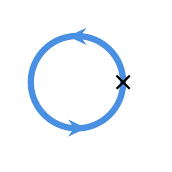
\begin{tikzpicture}[x=0.75pt,y=0.75pt,yscale=-0.8,xscale=0.8, baseline=(XXXX.south) ]
        \path (0,70);\path (69.33333587646484,0);\draw    ($(current bounding box.center)+(0,0.3em)$) node [anchor=south] (XXXX) {};
        %Shape: Circle [id:dp24884250139527841] 
        \draw  [color={rgb, 255:red, 74; green, 144; blue, 226 }  ,draw opacity=1 ][line width=2.25]  (1.47,32.64) .. controls (1.47,17.28) and (13.92,4.83) .. (29.28,4.83) .. controls (44.63,4.83) and (57.08,17.28) .. (57.08,32.64) .. controls (57.08,48) and (44.63,60.45) .. (29.28,60.45) .. controls (13.92,60.45) and (1.47,48) .. (1.47,32.64) -- cycle ;
        %Straight Lines [id:da5411158694039544] 
        \draw [color={rgb, 255:red, 74; green, 144; blue, 226 }  ,draw opacity=1 ]   (26.96,5.03) ;
        \draw [shift={(24.21,5.03)}, rotate = 360] [fill={rgb, 255:red, 74; green, 144; blue, 226 }  ,fill opacity=1 ][line width=0.08]  [draw opacity=0] (10.72,-5.15) -- (0,0) -- (10.72,5.15) -- (7.12,0) -- cycle    ;
        %Straight Lines [id:da9620266274824838] 
        \draw [color={rgb, 255:red, 74; green, 144; blue, 226 }  ,draw opacity=1 ]   (32.21,60.28) ;
        \draw [shift={(34.71,60.28)}, rotate = 180] [fill={rgb, 255:red, 74; green, 144; blue, 226 }  ,fill opacity=1 ][line width=0.08]  [draw opacity=0] (10.72,-5.15) -- (0,0) -- (10.72,5.15) -- (7.12,0) -- cycle    ;
        %Straight Lines [id:da020624625889882342] 
        \draw    (57.08,32.64) ;
        \draw [shift={(57.08,32.64)}, rotate = 45] [color={rgb, 255:red, 0; green, 0; blue, 0 }  ][line width=0.75]    (-5.59,0) -- (5.59,0)(0,5.59) -- (0,-5.59)   ;
        \end{tikzpicture}
        =\textcolor[rgb]{0.96,0.65,0.14}{\sum }\tikzset{every picture/.style={line width=0.75pt}} %set default line width to 0.75pt        
        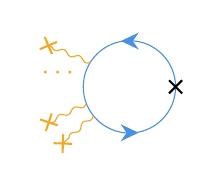
\begin{tikzpicture}[x=0.75pt,y=0.75pt,yscale=-0.8,xscale=0.8, baseline=(XXXX.south) ]
        \path (0,76);\path (100,0);\draw    ($(current bounding box.center)+(0,0.3em)$) node [anchor=south] (XXXX) {};
        %Shape: Circle [id:dp5911774442865243] 
        \draw  [color={rgb, 255:red, 74; green, 144; blue, 226 }  ,draw opacity=1 ] (33.47,35.64) .. controls (33.47,20.28) and (45.92,7.83) .. (61.28,7.83) .. controls (76.63,7.83) and (89.08,20.28) .. (89.08,35.64) .. controls (89.08,51) and (76.63,63.45) .. (61.28,63.45) .. controls (45.92,63.45) and (33.47,51) .. (33.47,35.64) -- cycle ;
        %Straight Lines [id:da2227266556401064] 
        \draw [color={rgb, 255:red, 74; green, 144; blue, 226 }  ,draw opacity=1 ]   (58.96,8.03) ;
        \draw [shift={(56.21,8.03)}, rotate = 360] [fill={rgb, 255:red, 74; green, 144; blue, 226 }  ,fill opacity=1 ][line width=0.08]  [draw opacity=0] (10.72,-5.15) -- (0,0) -- (10.72,5.15) -- (7.12,0) -- cycle    ;
        %Straight Lines [id:da7007234232463695] 
        \draw [color={rgb, 255:red, 74; green, 144; blue, 226 }  ,draw opacity=1 ]   (64.21,63.28) ;
        \draw [shift={(66.71,63.28)}, rotate = 180] [fill={rgb, 255:red, 74; green, 144; blue, 226 }  ,fill opacity=1 ][line width=0.08]  [draw opacity=0] (10.72,-5.15) -- (0,0) -- (10.72,5.15) -- (7.12,0) -- cycle    ;
        %Straight Lines [id:da8723273674088199] 
        \draw [color={rgb, 255:red, 245; green, 166; blue, 35 }  ,draw opacity=1 ]   (37.72,20.89) .. controls (35.55,21.82) and (34.01,21.2) .. (33.08,19.03) .. controls (32.15,16.86) and (30.61,16.24) .. (28.44,17.17) .. controls (26.27,18.1) and (24.73,17.48) .. (23.8,15.31) .. controls (22.87,13.14) and (21.32,12.52) .. (19.15,13.45) .. controls (16.98,14.38) and (15.44,13.76) .. (14.51,11.59) -- (12.46,10.77) -- (12.46,10.77) ;
        \draw [shift={(12.46,10.77)}, rotate = 246.84] [color={rgb, 255:red, 245; green, 166; blue, 35 }  ,draw opacity=1 ][line width=0.75]    (-5.59,0) -- (5.59,0)(0,5.59) -- (0,-5.59)   ;
        %Straight Lines [id:da9766871436629114] 
        \draw    (89.08,35.64) ;
        \draw [shift={(89.08,35.64)}, rotate = 45] [color={rgb, 255:red, 0; green, 0; blue, 0 }  ][line width=0.75]    (-5.59,0) -- (5.59,0)(0,5.59) -- (0,-5.59)   ;
        %Straight Lines [id:da08128573819662277] 
        \draw [color={rgb, 255:red, 245; green, 166; blue, 35 }  ,draw opacity=1 ]   (35.21,45.77) .. controls (34.46,48) and (32.97,48.75) .. (30.74,48) .. controls (28.5,47.25) and (27.01,48) .. (26.26,50.24) .. controls (25.51,52.47) and (24.02,53.22) .. (21.79,52.47) .. controls (19.55,51.72) and (18.06,52.47) .. (17.32,54.71) .. controls (16.58,56.95) and (15.09,57.7) .. (12.85,56.95) -- (12.71,57.02) -- (12.71,57.02) ;
        \draw [shift={(12.71,57.02)}, rotate = 198.43] [color={rgb, 255:red, 245; green, 166; blue, 35 }  ,draw opacity=1 ][line width=0.75]    (-5.59,0) -- (5.59,0)(0,5.59) -- (0,-5.59)   ;
        %Straight Lines [id:da9537702924229883] 
        \draw [color={rgb, 255:red, 245; green, 166; blue, 35 }  ,draw opacity=1 ]   (39.46,52.77) .. controls (39.37,55.12) and (38.15,56.26) .. (35.8,56.17) .. controls (33.45,56.09) and (32.23,57.23) .. (32.14,59.58) .. controls (32.05,61.93) and (30.83,63.07) .. (28.48,62.99) .. controls (26.13,62.91) and (24.91,64.05) .. (24.82,66.4) -- (21.21,69.77) -- (21.21,69.77) ;
        \draw [shift={(21.21,69.77)}, rotate = 182.03] [color={rgb, 255:red, 245; green, 166; blue, 35 }  ,draw opacity=1 ][line width=0.75]    (-5.59,0) -- (5.59,0)(0,5.59) -- (0,-5.59)   ;
        % Text Node
        \draw (6.75,22.5) node [anchor=north west][inner sep=0.75pt]  [color={rgb, 255:red, 245; green, 166; blue, 35 }  ,opacity=1 ] [align=left] {$\displaystyle \cdots $};
        \end{tikzpicture}
        }
    \]
    
    \uncover<4->{
        In the full $H^{\text{Floquet}}$, 
        automatically all PT terms are considered!
    }
}

\end{frame}

\begin{frame}
\frametitle{Floquet formalism v.s. RWA}

\vspace{0.3cm}
\begin{columns}

\begin{column}{0.6\textwidth}
\begin{minipage}{\columnwidth}
    \begin{center}
        \small
        \only<1>{
            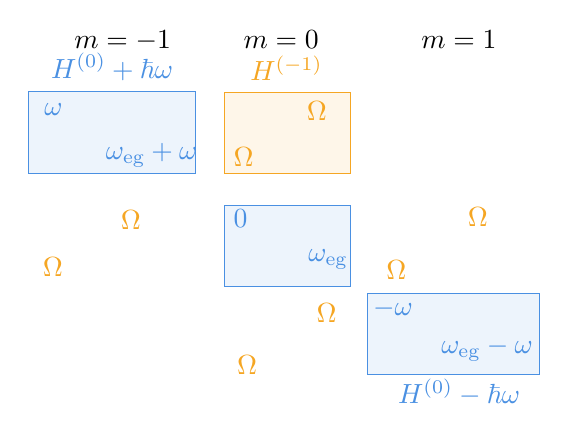
\begin{tikzpicture}[x=0.75pt,y=0.75pt,yscale=-0.8,xscale=0.8]
                %uncomment if require: \path (0,300); %set diagram left start at 0, and has height of 300
                
                %Shape: Rectangle [id:dp22527454007548142] 
                \draw  [color={rgb, 255:red, 74; green, 144; blue, 226 }  ,draw opacity=1 ][fill={rgb, 255:red, 74; green, 144; blue, 226 }  ,fill opacity=0.1 ] (139,112) -- (214.83,112) -- (214.83,160.95) -- (139,160.95) -- cycle ;
                %Shape: Rectangle [id:dp39605556332568703] 
                \draw  [color={rgb, 255:red, 74; green, 144; blue, 226 }  ,draw opacity=1 ][fill={rgb, 255:red, 74; green, 144; blue, 226 }  ,fill opacity=0.1 ] (225,165) -- (328.83,165) -- (328.83,213.95) -- (225,213.95) -- cycle ;
                %Shape: Rectangle [id:dp04514991260908907] 
                \draw  [color={rgb, 255:red, 74; green, 144; blue, 226 }  ,draw opacity=1 ][fill={rgb, 255:red, 74; green, 144; blue, 226 }  ,fill opacity=0.1 ] (20.83,43.81) -- (121.83,43.81) -- (121.83,92.95) -- (20.83,92.95) -- cycle ;
                %Shape: Rectangle [id:dp04085472927315914] 
                \draw  [color={rgb, 255:red, 245; green, 166; blue, 35 }  ,draw opacity=1 ][fill={rgb, 255:red, 245; green, 166; blue, 35 }  ,fill opacity=0.1 ] (138.83,44) -- (214.67,44) -- (214.67,92.95) -- (138.83,92.95) -- cycle ;
                
                % Text Node
                \draw (188,137) node [anchor=north west][inner sep=0.75pt]  [color={rgb, 255:red, 74; green, 144; blue, 226 }  ,opacity=1 ]  {$\omega _{\text{eg}}$};
                % Text Node
                \draw (143,113) node [anchor=north west][inner sep=0.75pt]  [color={rgb, 255:red, 74; green, 144; blue, 226 }  ,opacity=1 ]  {$0$};
                % Text Node
                \draw (187,48) node [anchor=north west][inner sep=0.75pt]  [color={rgb, 255:red, 245; green, 166; blue, 35 }  ,opacity=1 ]  {$\Omega $};
                % Text Node
                \draw (143,76) node [anchor=north west][inner sep=0.75pt]  [color={rgb, 255:red, 245; green, 166; blue, 35 }  ,opacity=1 ]  {$\Omega $};
                % Text Node
                \draw (66,73) node [anchor=north west][inner sep=0.75pt]  [color={rgb, 255:red, 74; green, 144; blue, 226 }  ,opacity=1 ]  {$\omega _{\text{eg}} +\omega $};
                % Text Node
                \draw (29,49) node [anchor=north west][inner sep=0.75pt]  [color={rgb, 255:red, 74; green, 144; blue, 226 }  ,opacity=1 ]  {$\omega $};
                % Text Node
                \draw (75,114) node [anchor=north west][inner sep=0.75pt]  [color={rgb, 255:red, 245; green, 166; blue, 35 }  ,opacity=1 ]  {$\Omega $};
                % Text Node
                \draw (28,142) node [anchor=north west][inner sep=0.75pt]  [color={rgb, 255:red, 245; green, 166; blue, 35 }  ,opacity=1 ]  {$\Omega $};
                % Text Node
                \draw (268,190) node [anchor=north west][inner sep=0.75pt]  [color={rgb, 255:red, 74; green, 144; blue, 226 }  ,opacity=1 ]  {$\omega _{\text{eg}} -\omega $};
                % Text Node
                \draw (227,167) node [anchor=north west][inner sep=0.75pt]  [color={rgb, 255:red, 74; green, 144; blue, 226 }  ,opacity=1 ]  {$-\omega $};
                % Text Node
                \draw (284,112) node [anchor=north west][inner sep=0.75pt]  [color={rgb, 255:red, 245; green, 166; blue, 35 }  ,opacity=1 ]  {$\Omega $};
                % Text Node
                \draw (235,144) node [anchor=north west][inner sep=0.75pt]  [color={rgb, 255:red, 245; green, 166; blue, 35 }  ,opacity=1 ]  {$\Omega $};
                % Text Node
                \draw (193,170) node [anchor=north west][inner sep=0.75pt]  [color={rgb, 255:red, 245; green, 166; blue, 35 }  ,opacity=1 ]  {$\Omega $};
                % Text Node
                \draw (145,201) node [anchor=north west][inner sep=0.75pt]  [color={rgb, 255:red, 245; green, 166; blue, 35 }  ,opacity=1 ]  {$\Omega $};
                % Text Node
                \draw (71.33,38.47) node [anchor=south] [inner sep=0.75pt]  [color={rgb, 255:red, 74; green, 144; blue, 226 }  ,opacity=1 ]  {$H^{( 0)} +\hbar \omega $};
                % Text Node
                \draw (280.33,224.77) node  [color={rgb, 255:red, 74; green, 144; blue, 226 }  ,opacity=1 ]  {$H^{( 0)} -\hbar \omega $};
                % Text Node
                \draw (176.33,38.47) node [anchor=south] [inner sep=0.75pt]  [color={rgb, 255:red, 245; green, 166; blue, 35 }  ,opacity=1 ]  {$H^{( -1)}$};
                
                % Text Node
                \draw (47,5.5) node [anchor=north west][inner sep=0.75pt]    {$m=-1$};
                % Text Node
                \draw (149,5.5) node [anchor=north west][inner sep=0.75pt]    {$m=0$};
                % Text Node
                \draw (256,5.5) node [anchor=north west][inner sep=0.75pt]    {$m=1$};
                \end{tikzpicture}
        }
        \only<2>{
            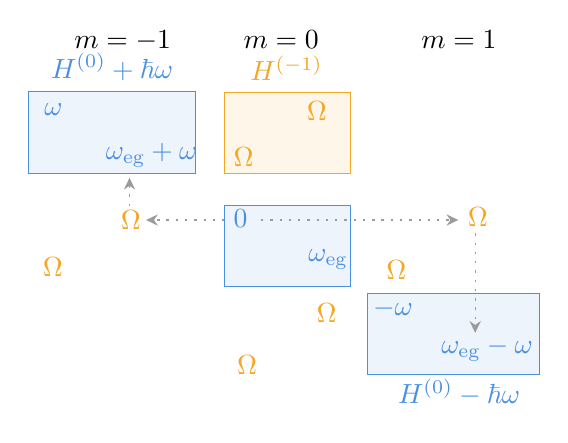
\begin{tikzpicture}[x=0.75pt,y=0.75pt,yscale=-0.8,xscale=0.8]
                %uncomment if require: \path (0,300); %set diagram left start at 0, and has height of 300
                
                %Shape: Rectangle [id:dp22527454007548142] 
                \draw  [color={rgb, 255:red, 74; green, 144; blue, 226 }  ,draw opacity=1 ][fill={rgb, 255:red, 74; green, 144; blue, 226 }  ,fill opacity=0.1 ] (139,112) -- (214.83,112) -- (214.83,160.95) -- (139,160.95) -- cycle ;
                %Shape: Rectangle [id:dp39605556332568703] 
                \draw  [color={rgb, 255:red, 74; green, 144; blue, 226 }  ,draw opacity=1 ][fill={rgb, 255:red, 74; green, 144; blue, 226 }  ,fill opacity=0.1 ] (225,165) -- (328.83,165) -- (328.83,213.95) -- (225,213.95) -- cycle ;
                %Straight Lines [id:da9943217194047385] 
                \draw [color={rgb, 255:red, 155; green, 155; blue, 155 }  ,draw opacity=1 ] [dash pattern={on 0.84pt off 2.51pt}]  (161,121) -- (276.83,121) ;
                \draw [shift={(279.83,121)}, rotate = 180] [fill={rgb, 255:red, 155; green, 155; blue, 155 }  ,fill opacity=1 ][line width=0.08]  [draw opacity=0] (7.14,-3.43) -- (0,0) -- (7.14,3.43) -- (4.74,0) -- cycle    ;
                %Straight Lines [id:da0017532091504999237] 
                \draw [color={rgb, 255:red, 155; green, 155; blue, 155 }  ,draw opacity=1 ] [dash pattern={on 0.84pt off 2.51pt}]  (290,129) -- (290,185.95) ;
                \draw [shift={(290,188.95)}, rotate = 270] [fill={rgb, 255:red, 155; green, 155; blue, 155 }  ,fill opacity=1 ][line width=0.08]  [draw opacity=0] (7.14,-3.43) -- (0,0) -- (7.14,3.43) -- (4.74,0) -- cycle    ;
                %Shape: Rectangle [id:dp04514991260908907] 
                \draw  [color={rgb, 255:red, 74; green, 144; blue, 226 }  ,draw opacity=1 ][fill={rgb, 255:red, 74; green, 144; blue, 226 }  ,fill opacity=0.1 ] (20.83,43.81) -- (121.83,43.81) -- (121.83,92.95) -- (20.83,92.95) -- cycle ;
                %Shape: Rectangle [id:dp04085472927315914] 
                \draw  [color={rgb, 255:red, 245; green, 166; blue, 35 }  ,draw opacity=1 ][fill={rgb, 255:red, 245; green, 166; blue, 35 }  ,fill opacity=0.1 ] (138.83,44) -- (214.67,44) -- (214.67,92.95) -- (138.83,92.95) -- cycle ;
                %Straight Lines [id:da9702765426343174] 
                \draw [color={rgb, 255:red, 155; green, 155; blue, 155 }  ,draw opacity=1 ] [dash pattern={on 0.84pt off 2.51pt}]  (139,121) -- (94.83,121) ;
                \draw [shift={(91.83,121)}, rotate = 360] [fill={rgb, 255:red, 155; green, 155; blue, 155 }  ,fill opacity=1 ][line width=0.08]  [draw opacity=0] (7.14,-3.43) -- (0,0) -- (7.14,3.43) -- (4.74,0) -- cycle    ;
                %Straight Lines [id:da49955628765150983] 
                \draw [color={rgb, 255:red, 155; green, 155; blue, 155 }  ,draw opacity=1 ] [dash pattern={on 0.84pt off 2.51pt}]  (81.83,112.61) -- (81.83,98.61) ;
                \draw [shift={(81.83,95.61)}, rotate = 90] [fill={rgb, 255:red, 155; green, 155; blue, 155 }  ,fill opacity=1 ][line width=0.08]  [draw opacity=0] (7.14,-3.43) -- (0,0) -- (7.14,3.43) -- (4.74,0) -- cycle    ;
                
                % Text Node
                \draw (188,137) node [anchor=north west][inner sep=0.75pt]  [color={rgb, 255:red, 74; green, 144; blue, 226 }  ,opacity=1 ]  {$\omega _{\text{eg}}$};
                % Text Node
                \draw (143,113) node [anchor=north west][inner sep=0.75pt]  [color={rgb, 255:red, 74; green, 144; blue, 226 }  ,opacity=1 ]  {$0$};
                % Text Node
                \draw (187,48) node [anchor=north west][inner sep=0.75pt]  [color={rgb, 255:red, 245; green, 166; blue, 35 }  ,opacity=1 ]  {$\Omega $};
                % Text Node
                \draw (143,76) node [anchor=north west][inner sep=0.75pt]  [color={rgb, 255:red, 245; green, 166; blue, 35 }  ,opacity=1 ]  {$\Omega $};
                % Text Node
                \draw (66,73) node [anchor=north west][inner sep=0.75pt]  [color={rgb, 255:red, 74; green, 144; blue, 226 }  ,opacity=1 ]  {$\omega _{\text{eg}} +\omega $};
                % Text Node
                \draw (29,49) node [anchor=north west][inner sep=0.75pt]  [color={rgb, 255:red, 74; green, 144; blue, 226 }  ,opacity=1 ]  {$\omega $};
                % Text Node
                \draw (75,114) node [anchor=north west][inner sep=0.75pt]  [color={rgb, 255:red, 245; green, 166; blue, 35 }  ,opacity=1 ]  {$\Omega $};
                % Text Node
                \draw (28,142) node [anchor=north west][inner sep=0.75pt]  [color={rgb, 255:red, 245; green, 166; blue, 35 }  ,opacity=1 ]  {$\Omega $};
                % Text Node
                \draw (268,190) node [anchor=north west][inner sep=0.75pt]  [color={rgb, 255:red, 74; green, 144; blue, 226 }  ,opacity=1 ]  {$\omega _{\text{eg}} -\omega $};
                % Text Node
                \draw (227,167) node [anchor=north west][inner sep=0.75pt]  [color={rgb, 255:red, 74; green, 144; blue, 226 }  ,opacity=1 ]  {$-\omega $};
                % Text Node
                \draw (284,112) node [anchor=north west][inner sep=0.75pt]  [color={rgb, 255:red, 245; green, 166; blue, 35 }  ,opacity=1 ]  {$\Omega $};
                % Text Node
                \draw (235,144) node [anchor=north west][inner sep=0.75pt]  [color={rgb, 255:red, 245; green, 166; blue, 35 }  ,opacity=1 ]  {$\Omega $};
                % Text Node
                \draw (193,170) node [anchor=north west][inner sep=0.75pt]  [color={rgb, 255:red, 245; green, 166; blue, 35 }  ,opacity=1 ]  {$\Omega $};
                % Text Node
                \draw (145,201) node [anchor=north west][inner sep=0.75pt]  [color={rgb, 255:red, 245; green, 166; blue, 35 }  ,opacity=1 ]  {$\Omega $};
                % Text Node
                \draw (71.33,38.47) node [anchor=south] [inner sep=0.75pt]  [color={rgb, 255:red, 74; green, 144; blue, 226 }  ,opacity=1 ]  {$H^{( 0)} +\hbar \omega $};
                % Text Node
                \draw (280.33,224.77) node  [color={rgb, 255:red, 74; green, 144; blue, 226 }  ,opacity=1 ]  {$H^{( 0)} -\hbar \omega $};
                % Text Node
                \draw (176.33,38.47) node [anchor=south] [inner sep=0.75pt]  [color={rgb, 255:red, 245; green, 166; blue, 35 }  ,opacity=1 ]  {$H^{( -1)}$};
                
                % Text Node
                \draw (47,5.5) node [anchor=north west][inner sep=0.75pt]    {$m=-1$};
                % Text Node
                \draw (149,5.5) node [anchor=north west][inner sep=0.75pt]    {$m=0$};
                % Text Node
                \draw (256,5.5) node [anchor=north west][inner sep=0.75pt]    {$m=1$};
                \end{tikzpicture}
        }
        \only<3>{
            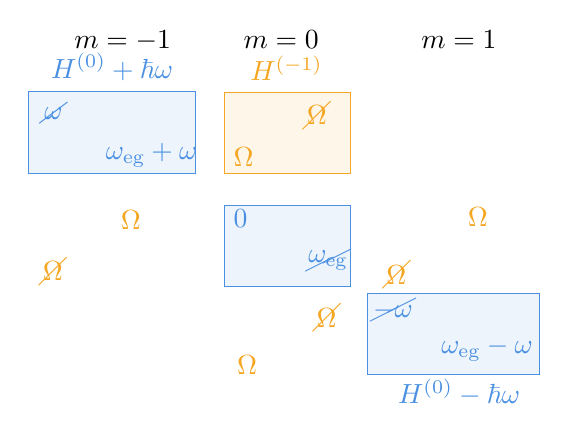
\begin{tikzpicture}[x=0.75pt,y=0.75pt,yscale=-0.8,xscale=0.8]
                %uncomment if require: \path (0,300); %set diagram left start at 0, and has height of 300
                
                %Shape: Rectangle [id:dp22527454007548142] 
                \draw  [color={rgb, 255:red, 74; green, 144; blue, 226 }  ,draw opacity=1 ][fill={rgb, 255:red, 74; green, 144; blue, 226 }  ,fill opacity=0.1 ] (139,112) -- (214.83,112) -- (214.83,160.95) -- (139,160.95) -- cycle ;
                %Shape: Rectangle [id:dp39605556332568703] 
                \draw  [color={rgb, 255:red, 74; green, 144; blue, 226 }  ,draw opacity=1 ][fill={rgb, 255:red, 74; green, 144; blue, 226 }  ,fill opacity=0.1 ] (225,165) -- (328.83,165) -- (328.83,213.95) -- (225,213.95) -- cycle ;
                %Shape: Rectangle [id:dp04514991260908907] 
                \draw  [color={rgb, 255:red, 74; green, 144; blue, 226 }  ,draw opacity=1 ][fill={rgb, 255:red, 74; green, 144; blue, 226 }  ,fill opacity=0.1 ] (20.83,43.81) -- (121.83,43.81) -- (121.83,92.95) -- (20.83,92.95) -- cycle ;
                %Shape: Rectangle [id:dp04085472927315914] 
                \draw  [color={rgb, 255:red, 245; green, 166; blue, 35 }  ,draw opacity=1 ][fill={rgb, 255:red, 245; green, 166; blue, 35 }  ,fill opacity=0.1 ] (138.83,44) -- (214.67,44) -- (214.67,92.95) -- (138.83,92.95) -- cycle ;
                
                % Text Node
                \draw (188,137) node [anchor=north west][inner sep=0.75pt]  [color={rgb, 255:red, 74; green, 144; blue, 226 }  ,opacity=1 ]  {$\cancel{\omega _{\text{eg}}}$};
                % Text Node
                \draw (143,113) node [anchor=north west][inner sep=0.75pt]  [color={rgb, 255:red, 74; green, 144; blue, 226 }  ,opacity=1 ]  {$0$};
                % Text Node
                \draw (187,48) node [anchor=north west][inner sep=0.75pt]  [color={rgb, 255:red, 245; green, 166; blue, 35 }  ,opacity=1 ]  {$\cancel{\Omega }$};
                % Text Node
                \draw (143,76) node [anchor=north west][inner sep=0.75pt]  [color={rgb, 255:red, 245; green, 166; blue, 35 }  ,opacity=1 ]  {$\Omega $};
                % Text Node
                \draw (66,73) node [anchor=north west][inner sep=0.75pt]  [color={rgb, 255:red, 74; green, 144; blue, 226 }  ,opacity=1 ]  {$\omega _{\text{eg}} +\omega $};
                % Text Node
                \draw (29,49) node [anchor=north west][inner sep=0.75pt]  [color={rgb, 255:red, 74; green, 144; blue, 226 }  ,opacity=1 ]  {$\cancel{\omega }$};
                % Text Node
                \draw (75,114) node [anchor=north west][inner sep=0.75pt]  [color={rgb, 255:red, 245; green, 166; blue, 35 }  ,opacity=1 ]  {$\Omega $};
                % Text Node
                \draw (28,142) node [anchor=north west][inner sep=0.75pt]  [color={rgb, 255:red, 245; green, 166; blue, 35 }  ,opacity=1 ]  {$\cancel{\Omega }$};
                % Text Node
                \draw (268,190) node [anchor=north west][inner sep=0.75pt]  [color={rgb, 255:red, 74; green, 144; blue, 226 }  ,opacity=1 ]  {$\omega _{\text{eg}} -\omega $};
                % Text Node
                \draw (227,167) node [anchor=north west][inner sep=0.75pt]  [color={rgb, 255:red, 74; green, 144; blue, 226 }  ,opacity=1 ]  {$\cancel{-\omega }$};
                % Text Node
                \draw (284,112) node [anchor=north west][inner sep=0.75pt]  [color={rgb, 255:red, 245; green, 166; blue, 35 }  ,opacity=1 ]  {$\Omega $};
                % Text Node
                \draw (235,144) node [anchor=north west][inner sep=0.75pt]  [color={rgb, 255:red, 245; green, 166; blue, 35 }  ,opacity=1 ]  {$\cancel{\Omega }$};
                % Text Node
                \draw (193,170) node [anchor=north west][inner sep=0.75pt]  [color={rgb, 255:red, 245; green, 166; blue, 35 }  ,opacity=1 ]  {$\cancel{\Omega }$};
                % Text Node
                \draw (145,201) node [anchor=north west][inner sep=0.75pt]  [color={rgb, 255:red, 245; green, 166; blue, 35 }  ,opacity=1 ]  {$\Omega $};
                % Text Node
                \draw (71.33,38.47) node [anchor=south] [inner sep=0.75pt]  [color={rgb, 255:red, 74; green, 144; blue, 226 }  ,opacity=1 ]  {$H^{( 0)} +\hbar \omega $};
                % Text Node
                \draw (280.33,224.77) node  [color={rgb, 255:red, 74; green, 144; blue, 226 }  ,opacity=1 ]  {$H^{( 0)} -\hbar \omega $};
                % Text Node
                \draw (176.33,38.47) node [anchor=south] [inner sep=0.75pt]  [color={rgb, 255:red, 245; green, 166; blue, 35 }  ,opacity=1 ]  {$H^{( -1)}$};
                
                % Text Node
                \draw (47,5.5) node [anchor=north west][inner sep=0.75pt]    {$m=-1$};
                % Text Node
                \draw (149,5.5) node [anchor=north west][inner sep=0.75pt]    {$m=0$};
                % Text Node
                \draw (256,5.5) node [anchor=north west][inner sep=0.75pt]    {$m=1$};
                \end{tikzpicture}
                  
        }
        \only<4>{
            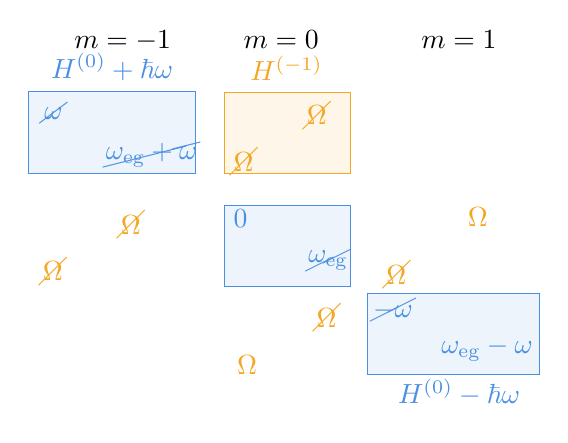
\begin{tikzpicture}[x=0.75pt,y=0.75pt,yscale=-0.8,xscale=0.8]
                %uncomment if require: \path (0,300); %set diagram left start at 0, and has height of 300
                
                %Shape: Rectangle [id:dp22527454007548142] 
                \draw  [color={rgb, 255:red, 74; green, 144; blue, 226 }  ,draw opacity=1 ][fill={rgb, 255:red, 74; green, 144; blue, 226 }  ,fill opacity=0.1 ] (139,112) -- (214.83,112) -- (214.83,160.95) -- (139,160.95) -- cycle ;
                %Shape: Rectangle [id:dp39605556332568703] 
                \draw  [color={rgb, 255:red, 74; green, 144; blue, 226 }  ,draw opacity=1 ][fill={rgb, 255:red, 74; green, 144; blue, 226 }  ,fill opacity=0.1 ] (225,165) -- (328.83,165) -- (328.83,213.95) -- (225,213.95) -- cycle ;
                %Shape: Rectangle [id:dp04514991260908907] 
                \draw  [color={rgb, 255:red, 74; green, 144; blue, 226 }  ,draw opacity=1 ][fill={rgb, 255:red, 74; green, 144; blue, 226 }  ,fill opacity=0.1 ] (20.83,43.81) -- (121.83,43.81) -- (121.83,92.95) -- (20.83,92.95) -- cycle ;
                %Shape: Rectangle [id:dp04085472927315914] 
                \draw  [color={rgb, 255:red, 245; green, 166; blue, 35 }  ,draw opacity=1 ][fill={rgb, 255:red, 245; green, 166; blue, 35 }  ,fill opacity=0.1 ] (138.83,44) -- (214.67,44) -- (214.67,92.95) -- (138.83,92.95) -- cycle ;
                
                % Text Node
                \draw (188,137) node [anchor=north west][inner sep=0.75pt]  [color={rgb, 255:red, 74; green, 144; blue, 226 }  ,opacity=1 ]  {$\cancel{\omega _{\text{eg}}}$};
                % Text Node
                \draw (143,113) node [anchor=north west][inner sep=0.75pt]  [color={rgb, 255:red, 74; green, 144; blue, 226 }  ,opacity=1 ]  {$0$};
                % Text Node
                \draw (187,48) node [anchor=north west][inner sep=0.75pt]  [color={rgb, 255:red, 245; green, 166; blue, 35 }  ,opacity=1 ]  {$\cancel{\Omega }$};
                % Text Node
                \draw (143,76) node [anchor=north west][inner sep=0.75pt]  [color={rgb, 255:red, 245; green, 166; blue, 35 }  ,opacity=1 ]  {$\cancel{\Omega }$};
                % Text Node
                \draw (66,73) node [anchor=north west][inner sep=0.75pt]  [color={rgb, 255:red, 74; green, 144; blue, 226 }  ,opacity=1 ]  {$\cancel{\omega _{\text{eg}} +\omega }$};
                % Text Node
                \draw (29,49) node [anchor=north west][inner sep=0.75pt]  [color={rgb, 255:red, 74; green, 144; blue, 226 }  ,opacity=1 ]  {$\cancel{\omega }$};
                % Text Node
                \draw (75,114) node [anchor=north west][inner sep=0.75pt]  [color={rgb, 255:red, 245; green, 166; blue, 35 }  ,opacity=1 ]  {$\cancel{\Omega }$};
                % Text Node
                \draw (28,142) node [anchor=north west][inner sep=0.75pt]  [color={rgb, 255:red, 245; green, 166; blue, 35 }  ,opacity=1 ]  {$\cancel{\Omega }$};
                % Text Node
                \draw (268,190) node [anchor=north west][inner sep=0.75pt]  [color={rgb, 255:red, 74; green, 144; blue, 226 }  ,opacity=1 ]  {$\omega _{\text{eg}} -\omega $};
                % Text Node
                \draw (227,167) node [anchor=north west][inner sep=0.75pt]  [color={rgb, 255:red, 74; green, 144; blue, 226 }  ,opacity=1 ]  {$\cancel{-\omega }$};
                % Text Node
                \draw (284,112) node [anchor=north west][inner sep=0.75pt]  [color={rgb, 255:red, 245; green, 166; blue, 35 }  ,opacity=1 ]  {$\Omega $};
                % Text Node
                \draw (235,144) node [anchor=north west][inner sep=0.75pt]  [color={rgb, 255:red, 245; green, 166; blue, 35 }  ,opacity=1 ]  {$\cancel{\Omega }$};
                % Text Node
                \draw (193,170) node [anchor=north west][inner sep=0.75pt]  [color={rgb, 255:red, 245; green, 166; blue, 35 }  ,opacity=1 ]  {$\cancel{\Omega }$};
                % Text Node
                \draw (145,201) node [anchor=north west][inner sep=0.75pt]  [color={rgb, 255:red, 245; green, 166; blue, 35 }  ,opacity=1 ]  {$\Omega $};
                % Text Node
                \draw (71.33,38.47) node [anchor=south] [inner sep=0.75pt]  [color={rgb, 255:red, 74; green, 144; blue, 226 }  ,opacity=1 ]  {$H^{( 0)} +\hbar \omega $};
                % Text Node
                \draw (280.33,224.77) node  [color={rgb, 255:red, 74; green, 144; blue, 226 }  ,opacity=1 ]  {$H^{( 0)} -\hbar \omega $};
                % Text Node
                \draw (176.33,38.47) node [anchor=south] [inner sep=0.75pt]  [color={rgb, 255:red, 245; green, 166; blue, 35 }  ,opacity=1 ]  {$H^{( -1)}$};
                
                % Text Node
                \draw (47,5.5) node [anchor=north west][inner sep=0.75pt]    {$m=-1$};
                % Text Node
                \draw (149,5.5) node [anchor=north west][inner sep=0.75pt]    {$m=0$};
                % Text Node
                \draw (256,5.5) node [anchor=north west][inner sep=0.75pt]    {$m=1$};
                \end{tikzpicture}                
        }
        \only<5>{
            \[
                H^{\text{RWA}} = \pmqty{
                    0 & \Omega \\ 
                    \Omega & \omegaeg - \omega
                }.
            \]
        }
    \end{center}
\end{minipage}
\end{column}

\begin{column}{0.5\textwidth}
    \begin{minipage}{\columnwidth}
        \centering
        \only<5>{
            $\abs*{\frac{E^{\text{Floquet}} - E^{\text{RWA}}}{E^{\text{Floquet}}}}$
            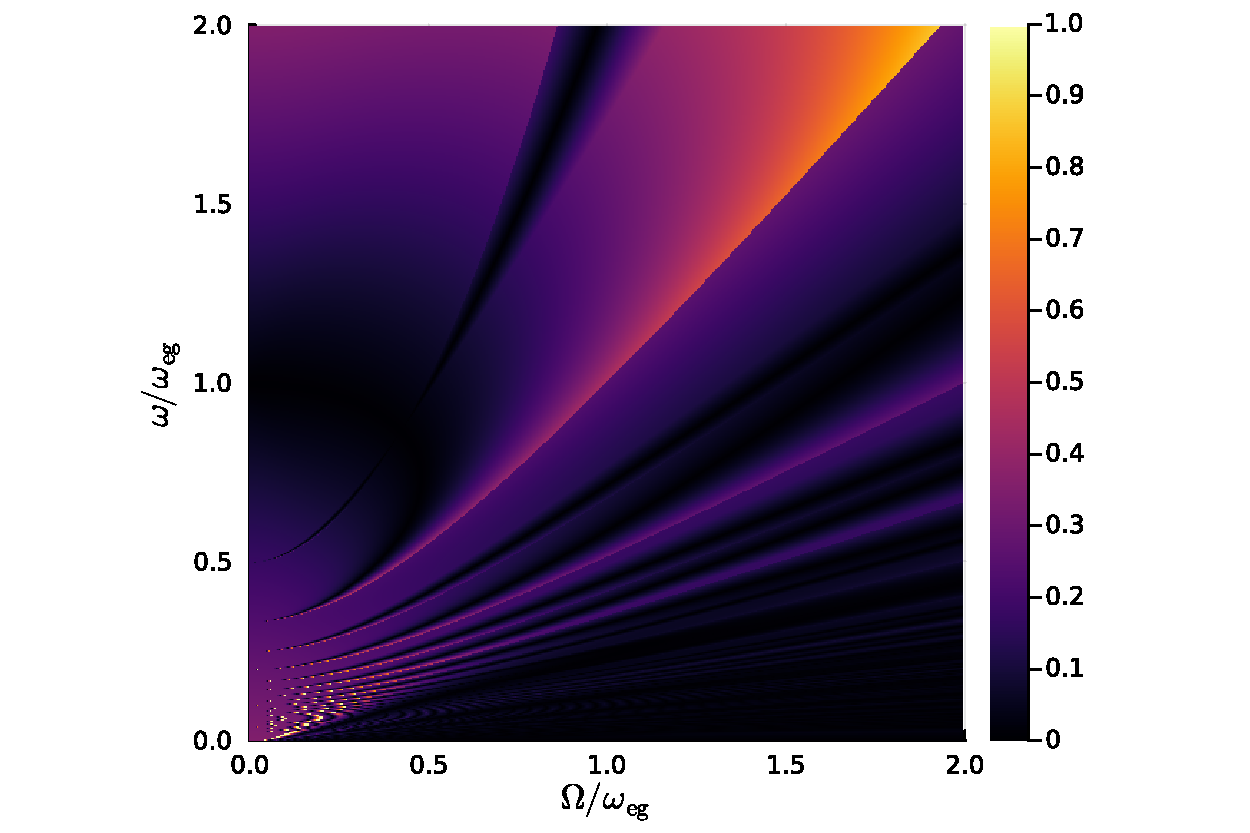
\includegraphics[width=\textwidth]{plot/relative-error-rwa.pdf} 
        }
    \end{minipage} 
\end{column}

\end{columns}

\vspace{-0.2cm}

\textbf{From Floquet to RWA}
\begin{itemize}
    \uncover<2->{\item Weak driving: first-order transitions from $\ket*{\text{g}^{ m=0}}$ dominates} 
    \uncover<4->{\item Near resonance: only $\ket*{\text{e}^{m=1}}$ ($\omegaeg - \omega$) matters}
\end{itemize}

\uncover<5>{Indeed when $\Omega / \omegaeg \lesssim 0.5$, $\omega / \omegaeg \sim 1$, RWA works the best!}

\end{frame}

\endgroup

\begingroup

\title{ARPES of Floquet systems}
\subtitle{Are Floquet states ``real''?}
\author{}
\date{}

\begin{frame}[noframenumbering,plain]
    \titlepage
\end{frame}

\begin{frame}
\frametitle{Angle-resolved photoemission spectroscopy (ARPES)}

\vspace{0.3cm}

\begin{columns}

\begin{column}{0.3\textwidth}
    \begin{minipage}{\columnwidth}
        ARPES sheds \emph{probe} beam to material (possibly \emph{pumped} by another beam) and detects output electrons' $(\vb{k}, E)$\footnote{
            Figure from \cite{rosenzweig2022surface}.
        }

    \end{minipage}
\end{column}

\begin{column}{0.7\textwidth}
\begin{minipage}{\columnwidth}
    \begin{center}
        \begin{tikzpicture}[x=0.75pt,y=0.75pt,yscale=-0.67,xscale=0.67]
            %uncomment if require: \path (0,300); %set diagram left start at 0, and has height of 300
            
            %Shape: Cube [id:dp3750648686000566] 
            \draw  [color={rgb, 255:red, 126; green, 211; blue, 33 }  ,draw opacity=1 ][fill={rgb, 255:red, 126; green, 211; blue, 33 }  ,fill opacity=0.5 ] (62,181.92) -- (103.55,140.38) -- (219,140.38) -- (219,145.45) -- (177.45,187) -- (62,187) -- cycle ; \draw  [color={rgb, 255:red, 126; green, 211; blue, 33 }  ,draw opacity=1 ] (219,140.38) -- (177.45,181.92) -- (62,181.92) ; \draw  [color={rgb, 255:red, 126; green, 211; blue, 33 }  ,draw opacity=1 ] (177.45,181.92) -- (177.45,187) ;
            %Straight Lines [id:da7634790971022005] 
            \draw [color={rgb, 255:red, 245; green, 166; blue, 35 }  ,draw opacity=1 ][line width=2.25]    (61,89.63) .. controls (63.33,89.97) and (64.33,91.31) .. (63.98,93.64) .. controls (63.63,95.97) and (64.62,97.31) .. (66.95,97.66) .. controls (69.28,98.01) and (70.28,99.35) .. (69.93,101.68) .. controls (69.58,104.01) and (70.58,105.35) .. (72.91,105.69) .. controls (75.24,106.04) and (76.23,107.38) .. (75.88,109.71) .. controls (75.53,112.04) and (76.53,113.38) .. (78.86,113.73) .. controls (81.19,114.08) and (82.19,115.42) .. (81.84,117.75) .. controls (81.49,120.08) and (82.48,121.41) .. (84.81,121.76) .. controls (87.14,122.11) and (88.14,123.45) .. (87.79,125.78) .. controls (87.44,128.11) and (88.44,129.45) .. (90.77,129.8) .. controls (93.1,130.15) and (94.09,131.49) .. (93.74,133.82) .. controls (93.39,136.15) and (94.39,137.49) .. (96.72,137.83) .. controls (99.05,138.18) and (100.05,139.52) .. (99.7,141.85) .. controls (99.35,144.18) and (100.34,145.52) .. (102.67,145.87) .. controls (105,146.22) and (106,147.56) .. (105.65,149.89) .. controls (105.3,152.22) and (106.3,153.56) .. (108.63,153.9) .. controls (110.96,154.25) and (111.95,155.59) .. (111.6,157.92) .. controls (111.25,160.25) and (112.25,161.59) .. (114.58,161.94) -- (116.67,164.75) -- (121.43,171.18) ;
            \draw [shift={(125,176)}, rotate = 233.46] [fill={rgb, 255:red, 245; green, 166; blue, 35 }  ,fill opacity=1 ][line width=0.08]  [draw opacity=0] (19.2,-4.8) -- (0,0) -- (19.2,4.8) -- cycle    ;
            %Straight Lines [id:da5392020227454484] 
            \draw  [dash pattern={on 4.5pt off 4.5pt}]  (125,63.38) -- (125,176) ;
            %Straight Lines [id:da31196217290539474] 
            \draw  [dash pattern={on 4.5pt off 4.5pt}]  (125,176) -- (214,176) ;
            %Shape: Polygon [id:ds7415407257771081] 
            \draw  [draw opacity=0][fill={rgb, 255:red, 74; green, 144; blue, 226 }  ,fill opacity=1 ] (175.93,60.54) -- (124.93,176.16) -- (155.93,53.54) -- cycle ;
            %Shape: Arc [id:dp6725542999955427] 
            \draw  [draw opacity=0] (207.58,68.31) .. controls (204.3,72.39) and (198.6,73.82) .. (193.84,71.43) .. controls (190.04,69.52) and (187.84,65.67) .. (187.78,61.62) -- (198.97,61.22) -- cycle ; \draw  [color={rgb, 255:red, 255; green, 255; blue, 255 }  ,draw opacity=1 ] (207.58,68.31) .. controls (204.3,72.39) and (198.6,73.82) .. (193.84,71.43) .. controls (190.04,69.52) and (187.84,65.67) .. (187.78,61.62) ;  
            %Shape: Ellipse [id:dp5480156492990544] 
            \draw  [draw opacity=0][fill={rgb, 255:red, 74; green, 178; blue, 226 }  ,fill opacity=1 ] (155.93,53.54) .. controls (157.38,49.13) and (163.08,47.06) .. (168.64,48.9) .. controls (174.21,50.74) and (177.53,55.81) .. (176.07,60.21) .. controls (174.62,64.62) and (168.92,66.69) .. (163.36,64.85) .. controls (157.79,63.01) and (154.47,57.94) .. (155.93,53.54) -- cycle ;
            %Straight Lines [id:da11942954119067473] 
            \draw [color={rgb, 255:red, 155; green, 155; blue, 155 }  ,draw opacity=1 ] [dash pattern={on 4.5pt off 4.5pt}]  (165.93,57.04) -- (165.93,161.38) ;
            %Shape: Arc [id:dp005400996226632371] 
            \draw  [draw opacity=0] (125.15,101.11) .. controls (129.47,100.25) and (134.05,100.33) .. (138.59,101.52) .. controls (140.21,101.94) and (141.76,102.49) .. (143.23,103.14) -- (131,130.54) -- cycle ; \draw  [color={rgb, 255:red, 155; green, 155; blue, 155 }  ,draw opacity=1 ] (125.15,101.11) .. controls (129.47,100.25) and (134.05,100.33) .. (138.59,101.52) .. controls (140.21,101.94) and (141.76,102.49) .. (143.23,103.14) ;  
            %Straight Lines [id:da11694313518633415] 
            \draw [color={rgb, 255:red, 155; green, 155; blue, 155 }  ,draw opacity=1 ] [dash pattern={on 4.5pt off 4.5pt}]  (165.93,161.38) -- (125,176) ;
            %Shape: Arc [id:dp8705048613091191] 
            \draw  [draw opacity=0] (151.72,166.31) .. controls (152.92,169.2) and (153.68,172.3) .. (153.92,175.54) -- (124,177.79) -- cycle ; \draw  [color={rgb, 255:red, 155; green, 155; blue, 155 }  ,draw opacity=1 ] (151.72,166.31) .. controls (152.92,169.2) and (153.68,172.3) .. (153.92,175.54) ;  
            %Straight Lines [id:da41162263584463266] 
            \draw [color={rgb, 255:red, 74; green, 144; blue, 226 }  ,draw opacity=1 ]   (265.65,176.99) -- (346.83,220.38) ;
            \draw [shift={(263,175.57)}, rotate = 28.12] [fill={rgb, 255:red, 74; green, 144; blue, 226 }  ,fill opacity=1 ][line width=0.08]  [draw opacity=0] (7.14,-3.43) -- (0,0) -- (7.14,3.43) -- (4.74,0) -- cycle    ;
            %Straight Lines [id:da5722111028183496] 
            \draw [color={rgb, 255:red, 74; green, 144; blue, 226 }  ,draw opacity=1 ]   (346.83,220.38) -- (434.02,188.41) ;
            \draw [shift={(436.83,187.38)}, rotate = 159.86] [fill={rgb, 255:red, 74; green, 144; blue, 226 }  ,fill opacity=1 ][line width=0.08]  [draw opacity=0] (7.14,-3.43) -- (0,0) -- (7.14,3.43) -- (4.74,0) -- cycle    ;
            %Straight Lines [id:da03447751310934799] 
            \draw [color={rgb, 255:red, 74; green, 144; blue, 226 }  ,draw opacity=1 ]   (436.83,176.38) -- (436.83,24.38) ;
            \draw [shift={(436.83,21.38)}, rotate = 90] [fill={rgb, 255:red, 74; green, 144; blue, 226 }  ,fill opacity=1 ][line width=0.08]  [draw opacity=0] (7.14,-3.43) -- (0,0) -- (7.14,3.43) -- (4.74,0) -- cycle    ;
            %Image [id:dp6464046109579271] 
            \draw (358.92,125.08) node  {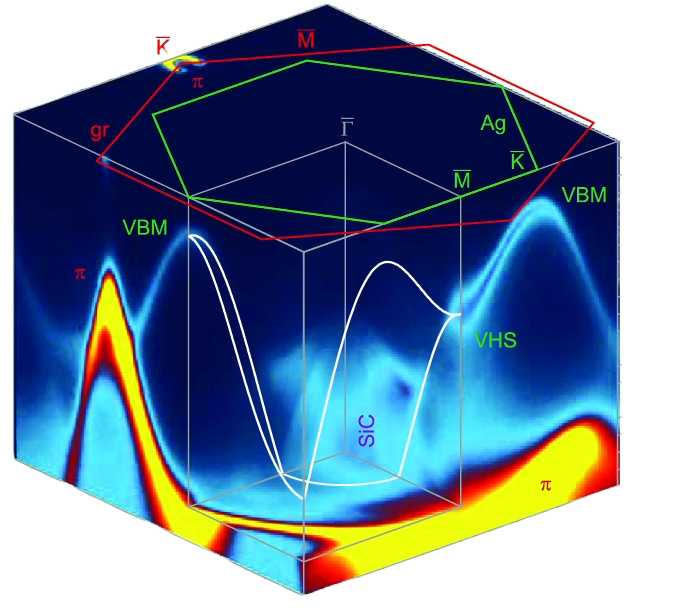
\includegraphics[width=0.4\textwidth]{plot/3D-ARPES-overview-of-the-graphene-Ag-SiC-heterostack-data-collected-at-room-temperature.png}};
            %Straight Lines [id:da8358864237885573] 
            \draw [color={rgb, 255:red, 226; green, 215; blue, 89 }  ,draw opacity=1 ][line width=2.25]    (37,30.29) .. controls (39.33,30.64) and (40.33,31.98) .. (39.98,34.31) .. controls (39.63,36.64) and (40.62,37.98) .. (42.95,38.33) .. controls (45.28,38.67) and (46.28,40.01) .. (45.93,42.34) .. controls (45.58,44.67) and (46.58,46.01) .. (48.91,46.36) .. controls (51.24,46.71) and (52.23,48.05) .. (51.88,50.38) .. controls (51.53,52.71) and (52.53,54.05) .. (54.86,54.4) .. controls (57.19,54.74) and (58.19,56.08) .. (57.84,58.41) .. controls (57.49,60.74) and (58.48,62.08) .. (60.81,62.43) .. controls (63.14,62.78) and (64.14,64.12) .. (63.79,66.45) .. controls (63.44,68.78) and (64.44,70.12) .. (66.77,70.47) .. controls (69.1,70.82) and (70.09,72.15) .. (69.74,74.48) .. controls (69.39,76.81) and (70.39,78.15) .. (72.72,78.5) .. controls (75.05,78.85) and (76.05,80.19) .. (75.7,82.52) .. controls (75.35,84.85) and (76.34,86.18) .. (78.67,86.53) .. controls (81,86.88) and (82,88.22) .. (81.65,90.55) .. controls (81.3,92.88) and (82.3,94.22) .. (84.63,94.57) .. controls (86.96,94.92) and (87.95,96.26) .. (87.6,98.59) .. controls (87.25,100.92) and (88.25,102.26) .. (90.58,102.6) -- (92.67,105.42) -- (97.43,111.85) ;
            \draw [shift={(101,116.67)}, rotate = 233.46] [fill={rgb, 255:red, 226; green, 215; blue, 89 }  ,fill opacity=1 ][line width=0.08]  [draw opacity=0] (19.2,-4.8) -- (0,0) -- (19.2,4.8) -- cycle    ;
            
            % Text Node
            \draw (131.5,97.54) node [anchor=south west] [inner sep=0.75pt]    {$\theta $};
            % Text Node
            \draw (171.5,171.6) node [anchor=south west] [inner sep=0.75pt]    {$\varphi $};
            % Text Node
            \draw (184.73,211.4) node [anchor=north] [inner sep=0.75pt]  [color={rgb, 255:red, 74; green, 144; blue, 226 }  ,opacity=1 ]  {$\mathbf{k}_{\parallel } =k(\sin \theta \cos \varphi ,\sin \theta \sin \varphi )$};
            % Text Node
            \draw (440.23,98.88) node [anchor=south] [inner sep=0.75pt]  [color={rgb, 255:red, 74; green, 144; blue, 226 }  ,opacity=1 ,rotate=-90]  {$E_{\text{kin, out}} -\omega _{0} +W$};
            % Text Node
            \draw (15.21,121.63) node [anchor=north west][inner sep=0.75pt]  [color={rgb, 255:red, 245; green, 166; blue, 35 }  ,opacity=1 ] [align=left] {pump \\(optional)};
            % Text Node
            \draw (65.33,26.96) node [anchor=north west][inner sep=0.75pt]  [color={rgb, 255:red, 226; green, 215; blue, 89 }  ,opacity=1 ] [align=left] {probe (much weaker)};
            
            
            \end{tikzpicture}                 
    \end{center}
\end{minipage}
\end{column}

\end{columns}

\vspace{0.1cm}

%\textbf{General form of ARPES signature}
\[
    \begin{aligned}
        &I_{\text{\scalebox{0.8}{\tiny \cite{chan2023}}}}(\vb{k}, \omega) \propto \underbrace{\int \dd{t_1} \int \dd{t_2} \ee^{\ii \omega (t_2 - t_1)} {\color[HTML]{E2D759} \abs*{M^{\text{dipole}}_{\text{probe}}}^2 } G^{{\color[HTML]{F5A623} \text{pumped}}, <}_{\vb{k}}(t_2, t_1)}_{\text{generalized Fermi golden rule for probing}} \\
        \Rightarrow & \boxed{I_{\text{Floquet}}(\vb{k}, \omega) \sim \sum_{n, m} \abs*{\phi_{n \vb{k}}^{(m)}}^2 \delta(\omega - \varepsilon_{n \vb{k}}).}
    \end{aligned}
\]


\end{frame}

\begin{frame}
\frametitle{ARPES for Floquet-driven electron bands}

\textbf{Three effects of Floquet correction to ARPES spectra}

\begin{columns}

\begin{column}{0.3\textwidth}
    \begin{minipage}{\columnwidth}
        In the figure:\footnote{
            Figure from \cite{zhou2023pseudospin}
        }
        \begin{itemize}
            \uncover<1->{\item Band replica: $H^{(0)} + m \hbar \omega$ }
            \uncover<2->{\item Intensity peak: $\abs*{\phi_n^{(m)}}^2$}
            \uncover<3->{\item Band renormalization: $H^{(m \neq 0)}$}
        \end{itemize}
    \end{minipage}
\end{column}

\begin{column}{0.7\textwidth}
    \begin{minipage}{\columnwidth}
        \begin{center}
            \begin{tikzpicture}[x=0.75pt,y=0.75pt,yscale=-1,xscale=1]
                %uncomment if require: \path (0,300); %set diagram left start at 0, and has height of 300
                
                %Image [id:dp8979975362917372] 
                \draw (122.83,124.5) node  {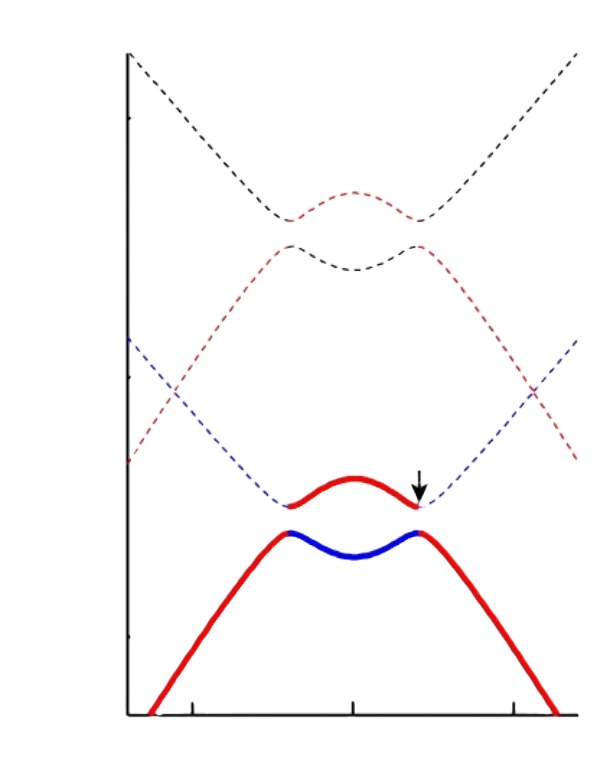
\includegraphics[width=190.25pt,height=190.25pt]{plot/arpes-band.png}};
                %Shape: Rectangle [id:dp9092995663180032] 
                \draw  [color={rgb, 255:red, 155; green, 155; blue, 155 }  ,draw opacity=1 ][dash pattern={on 0.84pt off 2.51pt}] (136,169.33) -- (158.33,169.33) -- (158.33,194.19) -- (136,194.19) -- cycle ;
                %Shape: Rectangle [id:dp13431941394505542] 
                \draw  [color={rgb, 255:red, 155; green, 155; blue, 155 }  ,draw opacity=1 ][dash pattern={on 0.84pt off 2.51pt}] (164.67,148.19) -- (187,148.19) -- (187,166.19) -- (164.67,166.19) -- cycle ;
                %Shape: Rectangle [id:dp3315405716067783] 
                \draw  [color={rgb, 255:red, 155; green, 155; blue, 155 }  ,draw opacity=1 ][dash pattern={on 0.84pt off 2.51pt}] (106,154.67) -- (128.33,154.67) -- (128.33,179.52) -- (106,179.52) -- cycle ;
                
                % Text Node
                \uncover<1->{\draw (138,197.19) node [anchor=north west][inner sep=0.75pt]   [align=left] {replica of bands};}
                % Text Node
                \uncover<2->{\draw (166.67,145.19) node [anchor=south west] [inner sep=0.75pt]   [align=left] {intensity variance\\from $\displaystyle |\phi _{n\mathbf{k}}^{( m)} |^{2}$};}
                % Text Node
                \uncover<3->{\draw (104,182.52) node [anchor=north east] [inner sep=0.75pt]   [align=left] {band \\renormalization};}
                
                
                \end{tikzpicture}        
        \end{center}
    \end{minipage}    
\end{column}

\end{columns}

\end{frame}

\begin{frame}
\frametitle{ARPES for Floquet-driven electron bands}

Probe at different stages of pump in topological insulator \ce{Bi2Se3} (\cite{mahmood2016selective})

\begin{center}
    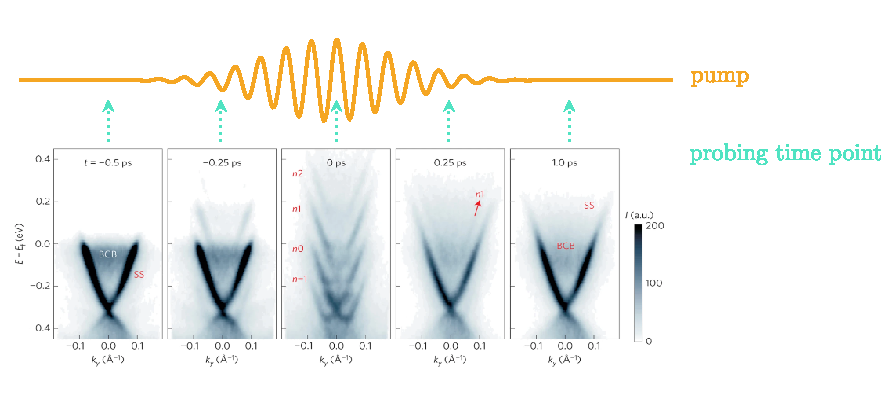
\includegraphics[width=0.99\textwidth]{plot/floquet-pump-relation.pdf}    
\end{center}

\only<1>{\textbf{Probe before the start of pump} nothing happens to ARPES spectrum} 
\only<2>{\textbf{Probe at the start of pump} mild Floquet features} 
\only<3>{\textbf{Probe at the middle of pump} Floquet}
\only<4>{\textbf{Probe at the tail of pump} mild Floquet features, plus signatures from usually unoccupied states}
\only<5>{\textbf{Probe after pump} signatures from usually unoccupied states}

\end{frame}

\begin{frame}
\frametitle{Self-driven Floquet effect}

Even after pump ends we may still see Floquet effects for excitonic materials like \ce{MoS2}\dots

\textbf{Floquet by exciton excited by pump -- \emph{self-driven} Floquet effects} (\cite{chan2023})

\begin{center}
    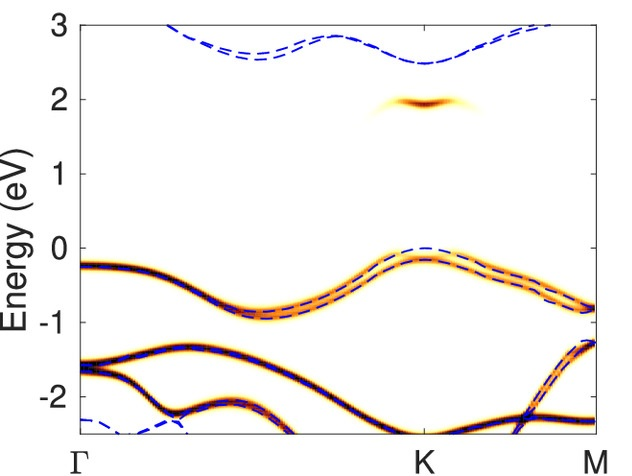
\includegraphics[width=0.5\textwidth]{plot/self-driven-floquet.jpg}
\end{center}

Dotted line: band structure without pumping

\end{frame}

\endgroup

\begin{frame}
\frametitle{Discussion}

\begin{itemize}
    \item Floquet quasienergies and quasi-stationary states 
    \item They are ``resummation'' of external field's perturbation
    \item They can be seen by ARPES!
\end{itemize}    

\end{frame}

\begin{frame}[allowframebreaks]
    \frametitle{References}

    \printbibliography

\end{frame}

\end{document}